%%%%%%%%%%%%%%%%%%%%%%%%%%%%%%%%%%%%%%%%%%%%%%%%%%%%%%%%%%%%%%%%%%%%
%% I, the copyright holder of this work, release this work into the
%% public domain. This applies worldwide. In some countries this may
%% not be legally possible; if so: I grant anyone the right to use
%% this work for any purpose, without any conditions, unless such
%% conditions are required by law.
%%%%%%%%%%%%%%%%%%%%%%%%%%%%%%%%%%%%%%%%%%%%%%%%%%%%%%%%%%%%%%%%%%%%

\documentclass[
  digital, %% The `digital` option enables the default options for the
           %% digital version of a document. Replace with `printed`
           %% to enable the default options for the printed version
           %% of a document.
%%  color,   %% Uncomment these lines (by removing the %% at the
%%           %% beginning) to use color in the digital version of your
%%           %% document
  table,   %% The `table` option causes the coloring of tables.
           %% Replace with `notable` to restore plain LaTeX tables.
  oneside, %% The `twoside` option enables double-sided typesetting.
           %% Use at least 120 g/m² paper to prevent show-through.
           %% Replace with `oneside` to use one-sided typesetting;
           %% use only if you don’t have access to a double-sided
           %% printer, or if one-sided typesetting is a formal
           %% requirement at your faculty.
  lof,     %% The `lof` option prints the List of Figures. Replace
           %% with `nolof` to hide the List of Figures.
  lot,     %% The `lot` option prints the List of Tables. Replace
           %% with `nolot` to hide the List of Tables.
  %% More options are listed in the user guide at
  %% <http://mirrors.ctan.org/macros/latex/contrib/fithesis/guide/mu/fi.pdf>.
]{fithesis3}
%% The following section sets up the locales used in the thesis.
\usepackage{polyglossia}  %% By using `czech` or `slovak` as the
\setmainlanguage{english} %% main locale instead of `english`, you
%% can typeset the thesis in either Czech or Slovak, respectively.
\setotherlanguages{czech} %% The
%% additional keys allow foreign texts to be typeset as follows:
%%
%%   \begin{otherlanguage}{german}  ... \end{otherlanguage}
%%   \begin{otherlanguage}{russian} ... \end{otherlanguage}
%%   \begin{otherlanguage}{czech}   ... \end{otherlanguage}
%%   \begin{otherlanguage}{slovak}  ... \end{otherlanguage}
%%
%% For non-Latin scripts, it may be necessary to load additional
%% fonts:
\newfontfamily\russianfont[Script=Cyrillic,Ligatures=TeX]{PT Serif}
%%
%% The following section sets up the metadata of the thesis.
\thesissetup{
    date        = \the\year/\the\month/\the\day,
    university  = mu,
    faculty     = fi,
    type        = bc,
    author      = Petr Janík,
    gender      = m,
    advisor     = {Ing. Lukáš Grolig},
    title       = {Receipt database with OCR scan},
    % TeXtitle    = {The Proof of $\mathsf{P}=\mathsf{NP}$},
    keywords    = {machine learning, OCR, React Native},
    % TeXkeywords = {keyword1, keyword2, \ldots},
    abstract    = {%
      This is the abstract of my thesis, which can

      span multiple paragraphs.
    },
    thanks      = {%
      I would like to thank my supervisor Ing. Lukáš Grolig for bringing up an incredibly interesting assignment for this thesis. 
      
      Secondly, I would like to acknowledge all my friends, family and colleagues who sent me images of receipts and took part in the survey.
      
      My biggest gratitude belongs to my girlfriend for her endless support, immense encouragement and countless advice.
    },
    bib         = example.bib,
    %% Uncomment the following line (by removing the %% at the
    %% beginning) and replace `assignment.pdf` with the filename
    %% of your scanned thesis assignment.
%%    assignment         = assignment.pdf,
}
\usepackage{makeidx}      %% The `makeidx` package contains
\makeindex                %% helper commands for index typesetting.
%% These additional packages are used within the document:
\usepackage{paralist} %% Compact list environments
\usepackage{amsmath}  %% Mathematics
\usepackage{amsthm}
\usepackage{amsfonts}
\usepackage{url}      %% Hyperlinks
\usepackage{markdown} %% Lightweight markup
\usepackage{tabularx} %% Tables
\usepackage{tabu}
\usepackage{booktabs}
\usepackage{listings} %% Source code highlighting
\lstset{
  basicstyle      = \ttfamily,
  identifierstyle = \color{black},
  keywordstyle    = \color{blue},
  keywordstyle    = {[2]\color{cyan}},
  keywordstyle    = {[3]\color{olive}},
  stringstyle     = \color{teal},
  commentstyle    = \itshape\color{magenta},
  breaklines      = true,
}
\usepackage{floatrow} %% Putting captions above tables
\floatsetup[table]{capposition=top}

% provides subfigure environment
\usepackage{subcaption}

% https://cs.overleaf.com/learn/latex/Code_Highlighting_with_minted
\usepackage{minted}
\usepackage{xcolor}
%\usemintedstyle{manni}
%\definecolor{bg}{rgb}{0.1,0.1,0.1}
\newcommand{\code}[1]{\mintinline[]{javascript}|#1|} % TODO change to jsx and compile locally using 'latexmk -lualatex fi-lualatex.tex' for jsx syntax support (https://tex.stackexchange.com/a/519333)

% Control inline code background dimensions
% https://tex.stackexchange.com/a/276750
% \usepackage{xpatch}

% \newlength{\mintedfboxsep}
% \setlength{\mintedfboxsep}{0.5pt}

% \makeatletter
% \newlength{\fboxrsep}
% \setlength{\fboxrsep}{\fboxsep}

% \newlength{\fboxlsep}
% \setlength{\fboxlsep}{\fboxsep}

% \newlength{\fboxtsep}
% \setlength{\fboxtsep}{\fboxsep}

% \newlength{\fboxbsep}
% \setlength{\fboxbsep}{\mintedfboxsep}

% \xpatchcmd{\minted@inputpyg@inline}{%
%   \colorbox%
% }{%
%   \long\def\color@b@x##1##2##3%
%   {\leavevmode
%     \setbox\z@\hbox{\kern\fboxlsep{\set@color##3}\kern\fboxrsep}%
%     \dimen@\ht\z@\advance\dimen@\fboxtsep\ht\z@\dimen@
%     \dimen@\dp\z@\advance\dimen@\fboxbsep\dp\z@\dimen@
%     {##1{##2\color@block{\wd\z@}{\ht\z@}{\dp\z@}\box\z@}}}%
%   \colorbox%
% }{\typeout{Success}}{\typeout{Failure}}
% \makeatother
% END of 'control inline code background dimensions'

% write thousand comma separator in numbers by wrapping them inside \num{}
\usepackage{siunitx}
\sisetup{group-separator={,}}

% do not wrap equations
\binoppenalty=\maxdimen
\relpenalty=\maxdimen

% add command to create inline color boxes
\makeatletter
\def\testclr#1#{\@testclr{#1}}
\def\@testclr#1#2{{\fboxsep\z@\fbox{\colorbox#1{#2}{\phantom{XX}}}}}
\makeatother

% silence some warnings
\usepackage{silence}
\WarningFilter{biblatex}{File 'american-iso.lbx' not found!}
\WarningFilter{caption}{Cannot determine current font size.}
\WarningFilter{latex}{year field}


\begin{document}
\chapter*{Introduction}
\addcontentsline{toc}{chapter}{Introduction}
\chapter*{Introduction}
During everyday life, people take part in transactions. Be it grocery shopping or refuelling of a car. Despite more and more goods being offered online, offline transactions still form an important part of the overall purchases. Proof of such transactions is, in most cases, a receipt. This proof is necessary when complaining or returning goods. However, it can get tough to keep track of all the receipts, and people can be rejected when asking for a refund simply because they either did not keep their receipt or put it among all the other receipts and are unable to find it. The receipt can also get damaged in such a way that it is not readable anymore. 

% a photo of a receipt is legally enough
The goal of my thesis is to develop an application that would serve as a user's digital receipt database. It would allow the user to take a photo of a receipt and by using optical character recognition it would extract the textual information from the photo. This extracted information would be used to prefill the receipt record. The receipt records should be editable and searchable, e.g. by the merchant name or items bought. The application should be available on Android and Windows.

In the first chapter, I provide a brief overview of techniques used for data extraction from images.

In the second chapter, I describe currently available applications that are trying to solve this task, their main features and drawbacks.

The next chapter is concerned with choosing the right technology for developing a cross-platform application. This chapter also provides an overview of the chosen framework – React Native.

An essential part of the thesis is testing and continuous integration. The types of testing that were used to ensure the high quality and reliability of the application are described in the fourth chapter.

The fifth chapter describes the functionality of the application. It shows how Microsoft Form Recognizer \cite{WhatIsFormRecognizer} was used to extract the information from a photo of a receipt. This chapter also includes a description of a receipt item categorization using word embeddings. The image processing using the OpenCV\footnote{\url{https://opencv.org/}} library is contained as well.

% compared to other applications
The last chapter provides an evaluation of the application: how well it extracts the data from the photo, how accurate the assigned item categories are and how well it processed the original photo to reduce the noise.

The outcome of the thesis is an application named Receipts Scanner. It can be used as a way to conveniently organize receipts and access them both from mobile and desktop. The patterns used in this application can be used for developing other React Native applications. 

\chapter{Image data extraction}

On a high level, the data extraction from the photo of a receipt involves two steps. 

\section{Optical character recognition}\index{OCR}
First, the raw text data need to be extracted. This is done using Optical Character Recognition (OCR). OCR is the process of translating images of handwritten, typewritten, or printed text into a format understood by machines. 
It works by pre-processing the image\footnote{Image pre-processing refers to a set of techniques, that are applied on the image to make it more suitable for the subsequent steps, e.g. by noise reduction.} and segmenting the text into lines, then words and eventually into individual characters to which a code, such as ASCII, is assigned. \cite{OCRCNN}

The code can be assigned based on template matching. An image of an unknown character is compared to a set of images of known characters. The code of the most similar character is chosen. The similarity can be computed e.g. as a difference between grayscale value of a pixel of the unknown character and a grayscale value of a pixel of the known character \cite{Ziegaus2016TemplateMatching}.
This approach works well\cite{Ziegaus2016TemplateMatching} for receipts, because the characters are printed by a computer and usually in the same font. 

Another approach is to extract the most relevant information from the character image. This is called feature extraction. An example of such feature could be a density of dark pixels in given part of the image. These features are used as inputs for machine learning models such as K-Nearest Neighbour a Support Vector Machines. \cite{singh2011feature}

The third approach is to use a Convolutional
Neural Network. It has the highest computational cost among the three mentioned approaches and requires a large dataset of images of characters to learn on, but it has the best performance. \cite{OCRCNN}

\section{Classifying data}
The second step is to assign a meaning to the parts of the extracted text. This can be done by pattern matching, dictionary matching or using more complex methods such as neural networks. 

Pattern matching makes use of the fact, that some data have a specific format compared to other data available on the receipt. For example dates and phone numbers can be extracted using regular expressions.

Dictionary matching tries to find a value from a list of possible values. An example would be finding a merchant name in a pre-defined list of merchants.

All methods can take advantage of the actual text position. The merchant name is most likely to appear on the top, the items in the middle and the total price at the bottom. However, receipts vary significantly in the locations of different data. Therefore this method, referred to as Zone OCR, is more suitable for forms and invoices where the format is known.

\chapter{Existing solutions}

Applications addressing this issue are usually referred to as expense managers. The most popular expense manager for iOS is called Smart Receipts\footnote{Smart Receipts homepage: \url{https://www.smartreceipts.co/}}. It is also available on Android, but it is superseded by an application called Receipt Scanner\footnote{Receipt Scanner on Google Play: \url{https://play.google.com/store/apps/details?id=com.easyexpense/}} in terms of downloads. They allow users to take photos of receipts and fill in additional information such as total price, date of purchase or expense category. These receipts can then be searched by name, price or category. Both applications provide an option to organize expenses into reports. User can then export these reports in CSV format; Smart Receipts also supports PDF export. Another feature is a visualization of expenses throughout time and across categories.

The main feature I will focus on is the automatic information extraction from the receipts. It is available for \$0.1 per scan in Smart Receipts (as of April 2021), and it is free in Receipt Scanner. Other applications that offer this feature are Expensify\footnote{Expensify on App Store: \url{https://apps.apple.com/au/app/expensify-receipts-expenses/id471713959}}, Receipt Lens\footnote{Receipt Lens on App Store: \url{https://apps.apple.com/us/app/receipt-lens-receipt-scanner/id1424280764}} and Dext\footnote{Dext on App Store: \url{https://apps.apple.com/us/app/dext-finance-and-accounting/id418327708}}. All are available for Android and iOS. The amount of information extracted from the picture is, however, limited. Usually, it includes only merchant name, total paid amount, tax amount, date, currency and category. Any information about individual items is missing.

An open source\footnote{Open source software is a software, whose source code is released with a permission to use, copy, distribute and modify. It is usually free to use. It is often developed collaboratively on platforms such as GitHub.} alternative to the mentioned applications is Receipt Manager\footnote{Receipt Manager on GitHub: \url{https://github.com/ReceiptManager}}.
It uses Tesseract\footnote{Tesseract on GitHub: https://github.com/tesseract-ocr/tesseract} for OCR and a fixed set of rules to extract the information. 
The main idea of this project is that it does not rely on any third-party services. It is available on iOS, Android and web. All these clients connect to a server on which the OCR runs. It is deployed separately as a Docker container.

\chapter{Authentication}
\textit{Authentication is the process of verifying an entity’s identity, given its credentials}\cite{Cankaya2011}.
For Receipts Scanner, user is the entity that is being authenticated.

The authentication in the application serves two purposes. The first one is the ability of connecting saved receipts with the user who created them. The second reason for authentication is to ensure proper database rules. The rules are set in such a way, that only authenticated user is able to create a new \textit{User} document. The user is able to read and modify the \textit{User} document if they are authenticated and if the document belongs to them. The last rule ensures, that each user is able to create, read and modify only their own receipts inside the \textit{Receipts} collection.

\begin{figure}
\centering
\begin{subfigure}[t]{0.5\textwidth}
  \centering
  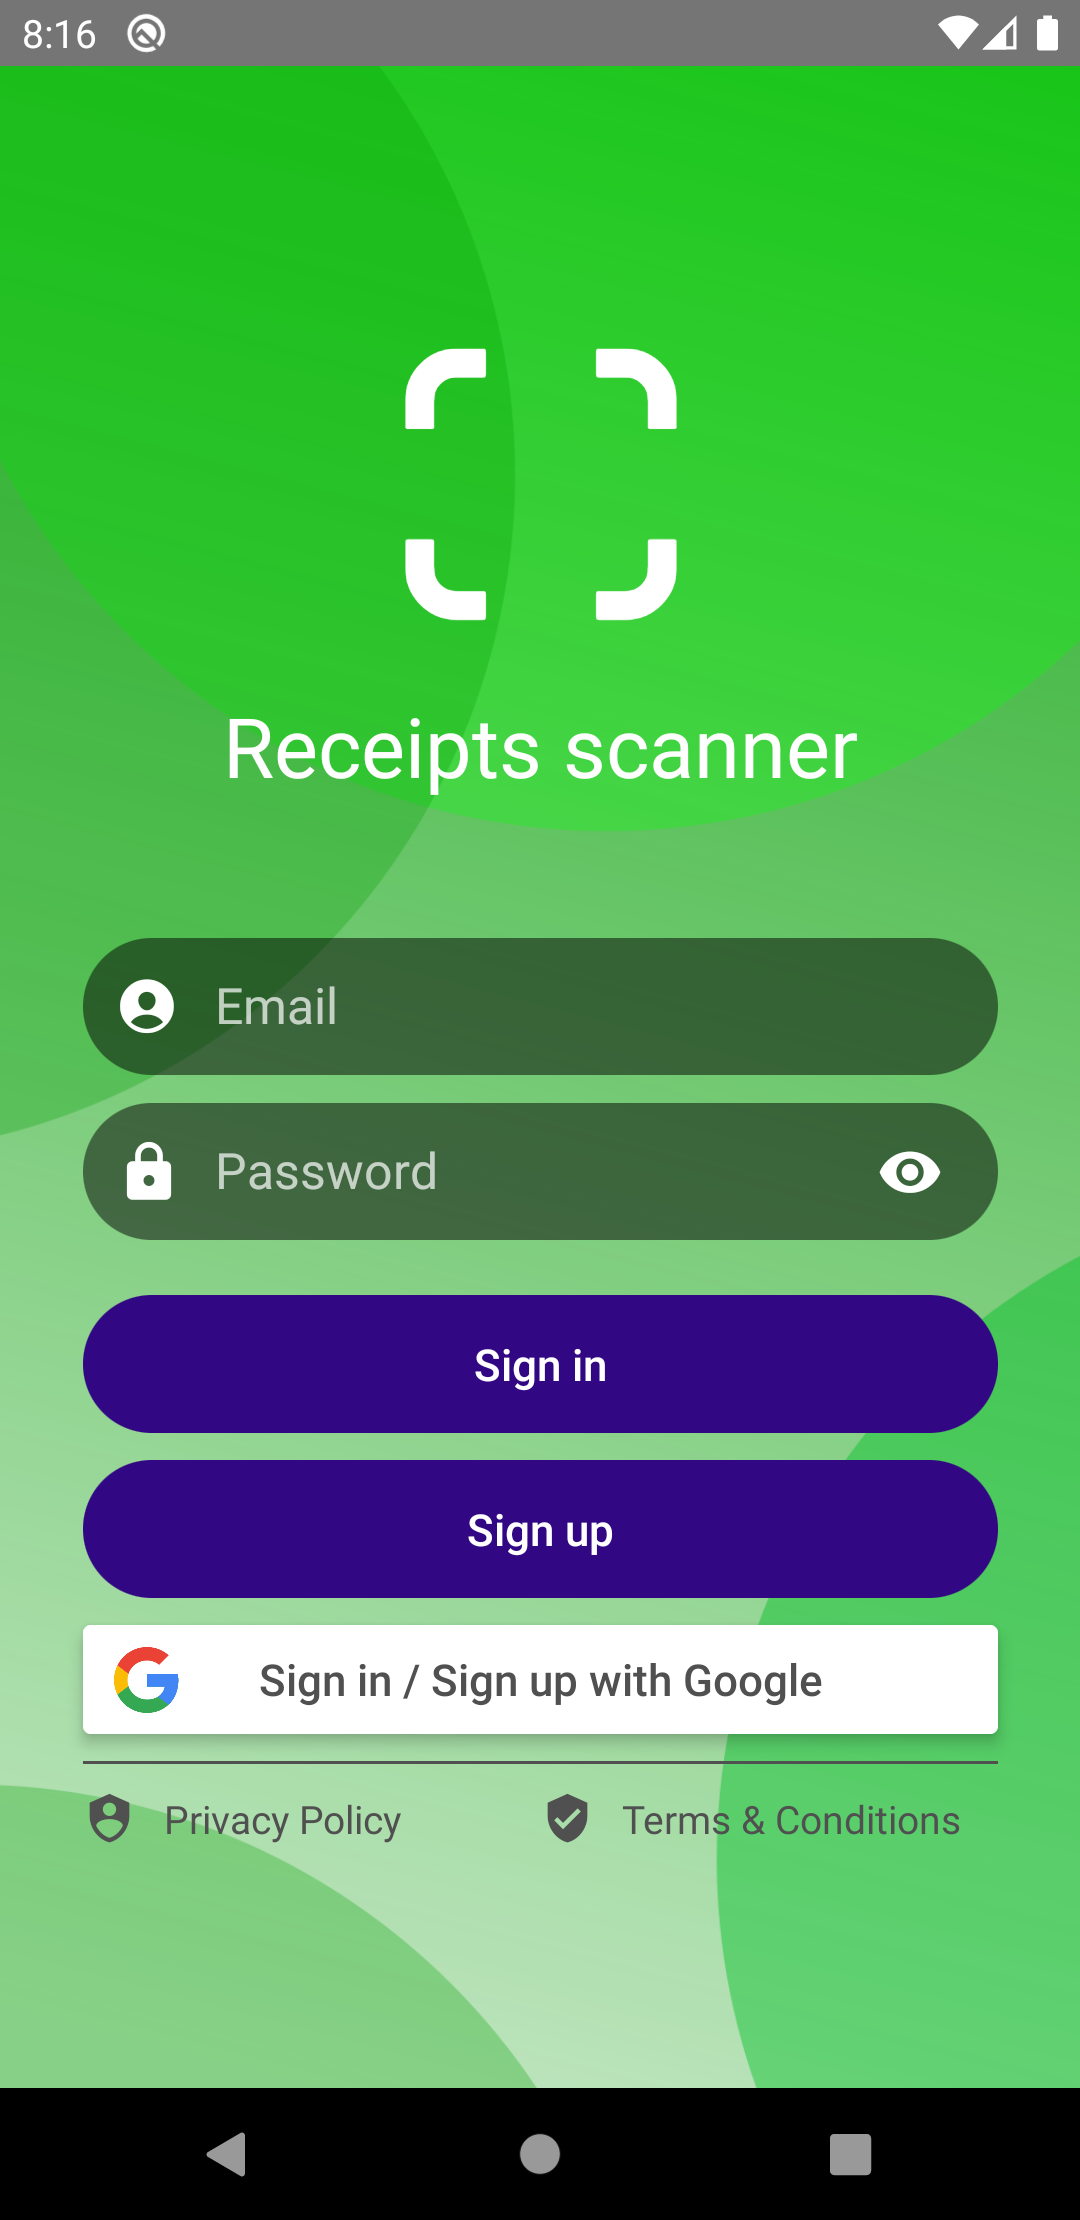
\includegraphics[width=0.95\textwidth]{figures/screens/android/light/login_screen}
  \caption{Empty login form.}
  \label{fig:login_screen}
\end{subfigure}
\begin{subfigure}[t]{0.5\textwidth}
  \centering
  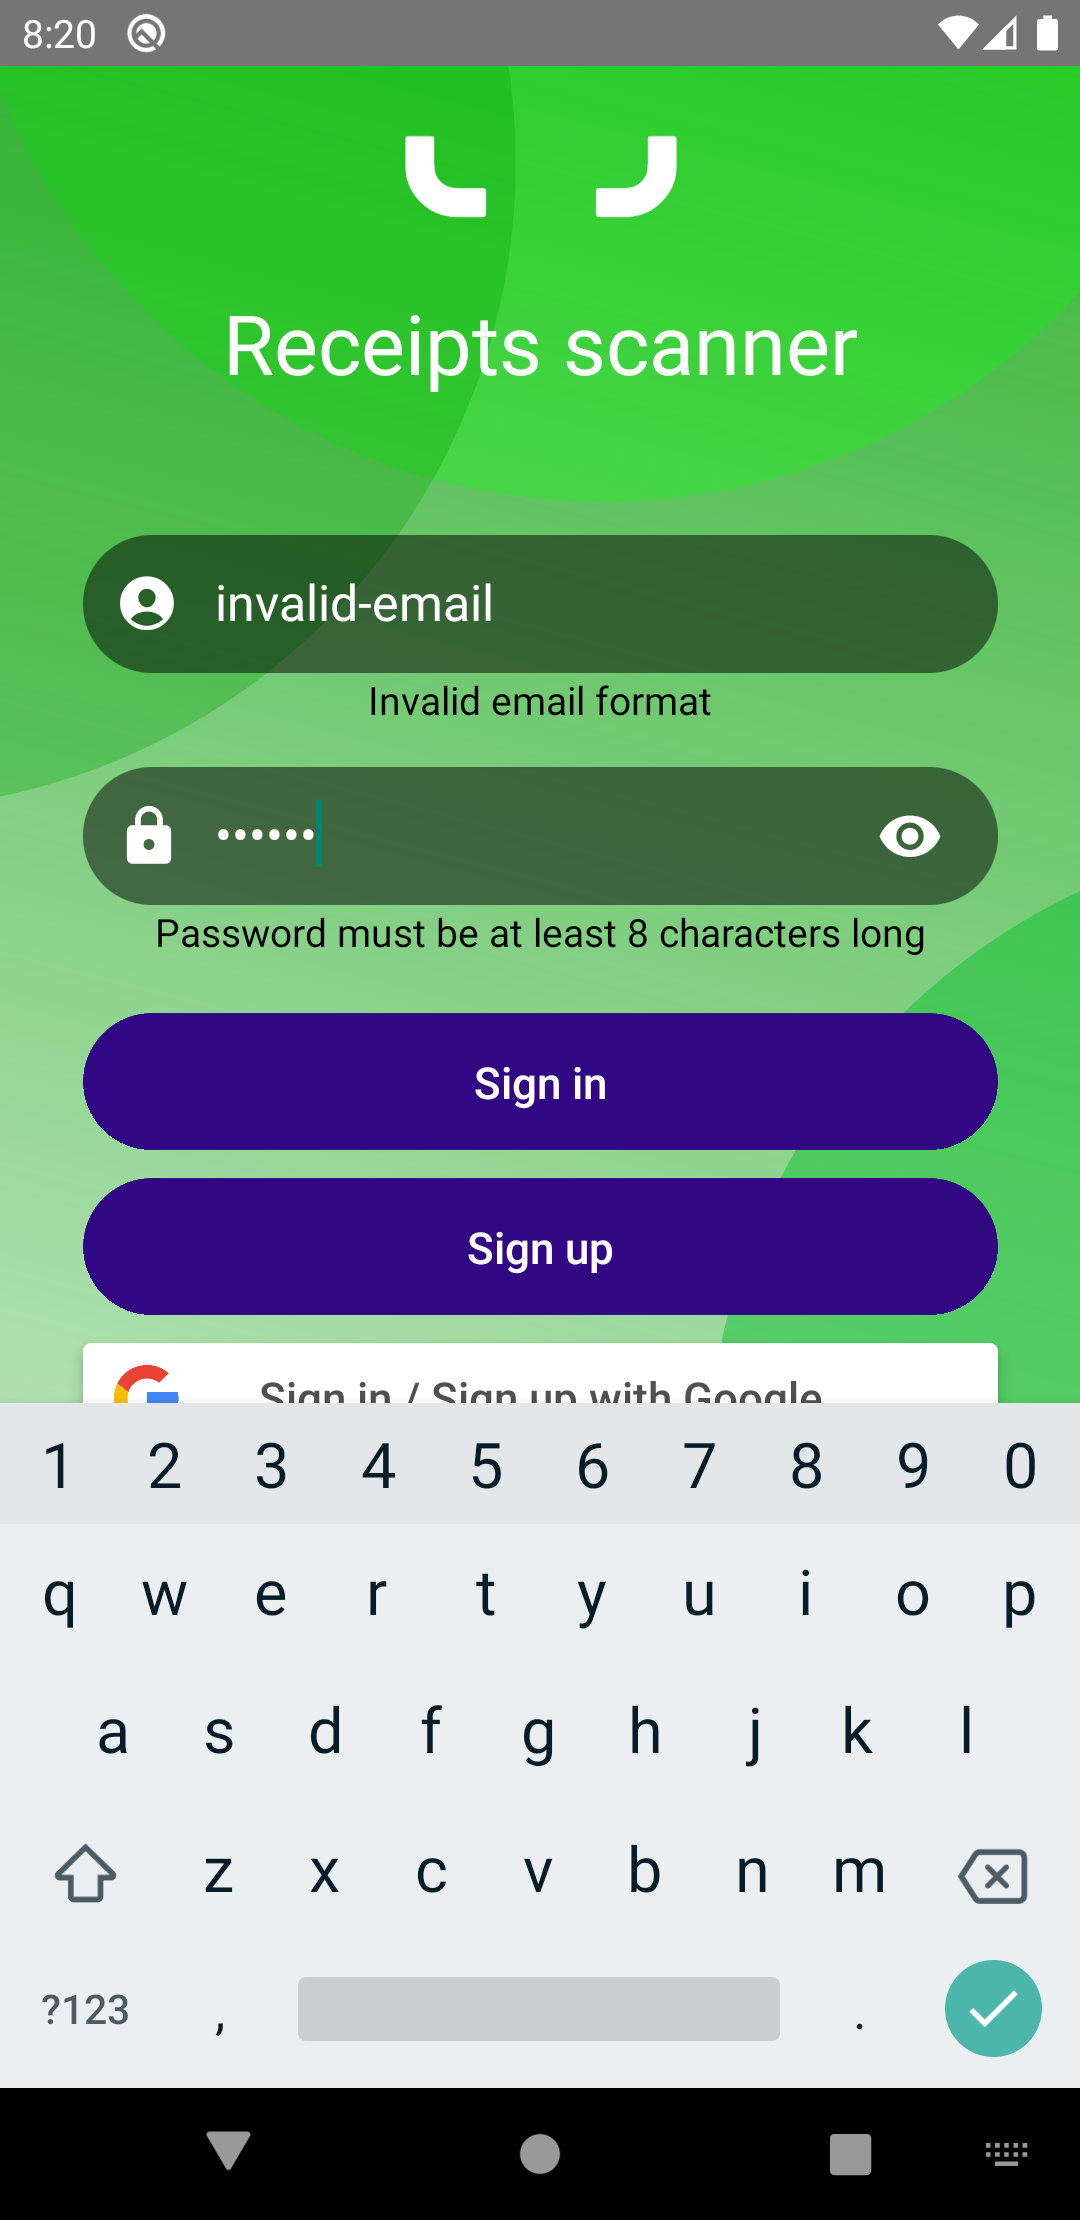
\includegraphics[width=0.95\textwidth]{figures/screens/android/light/login_validation}
  \caption{Form with validation errors.}
  \label{fig:login_validation}
\end{subfigure}
\caption{Login screen.}
\end{figure}

When the user first launches the application, a login screen is displayed. The Login screen is depicted in Figure \ref{fig:login_screen}. It consists of two text input fields and three buttons. The first input field is for email and the second is for password. It is possible to display the entered password in a clear-text form by pressing the eye icon next to the password input. Based on the user's preference they can choose one of the two supported authentication mechanisms:
\begin{enumerate}
    \item \textbf{Authentication with email and password}
    
    Figure \ref{fig:sign_in_flow} shows how the process of a sign-in using email and password looks. The form offers a real-time validation, so the user is instantly notified in case they have entered an invalid email or a password. The validation is show in Figure \ref{fig:login_validation}.
    
    \begin{figure}
        \begin{center}
            \includegraphics[width=\textwidth]{figures/diagrams/Sign_in_flow}
        \end{center}
        \caption{Activity diagram of a user signing in.}
        \label{fig:sign_in_flow}
    \end{figure}
    
    Figure \ref{fig:sign_up_flow} shows how the process of a sign-up using email and password looks.
    
    \begin{figure}
        \begin{center}
            \includegraphics[width=\textwidth]{figures/diagrams/Sign_up_flow}
        \end{center}
        \caption{Activity diagram of a user signing up.}
        \label{fig:sign_up_flow}
    \end{figure}
    
    \item \textbf{Authentication with a Google account}
    
    Figure \ref{fig:google_auth_flow} shows authentication flow using Google Sign In\footnote{GitHub repository of Google Sign In library: \url{https://github.com/react-native-google-signin/google-signin}} native module.
    Authentication with Google is not available on the Windows version of an application, because the Google Sign In library does not support React Native Windows yet\footnote{GitHub issue that tracks adding of support of Google Sign In for Windows: \url{https://github.com/microsoft/react-native-windows/issues/6531}}.
    
    \begin{figure}
        \begin{center}
            \includegraphics[width=0.9\textwidth]{figures/diagrams/Google_auth_flow}
        \end{center}
        \caption{Activity diagram of a user authenticating with a Google account.}
        \label{fig:google_auth_flow}
    \end{figure}
\end{enumerate}

A common property of all three mentioned workflows is that the user's session is persisted even if the application is restarted.

If a user wanted to use a different account they could sign out on the Settings screen, which is depicted in Figure \ref{fig:settings_screen}. Clicking the ``Sign out'' button ends the session and redirects the user back to the Login screen.

\begin{figure}
    \begin{center}
        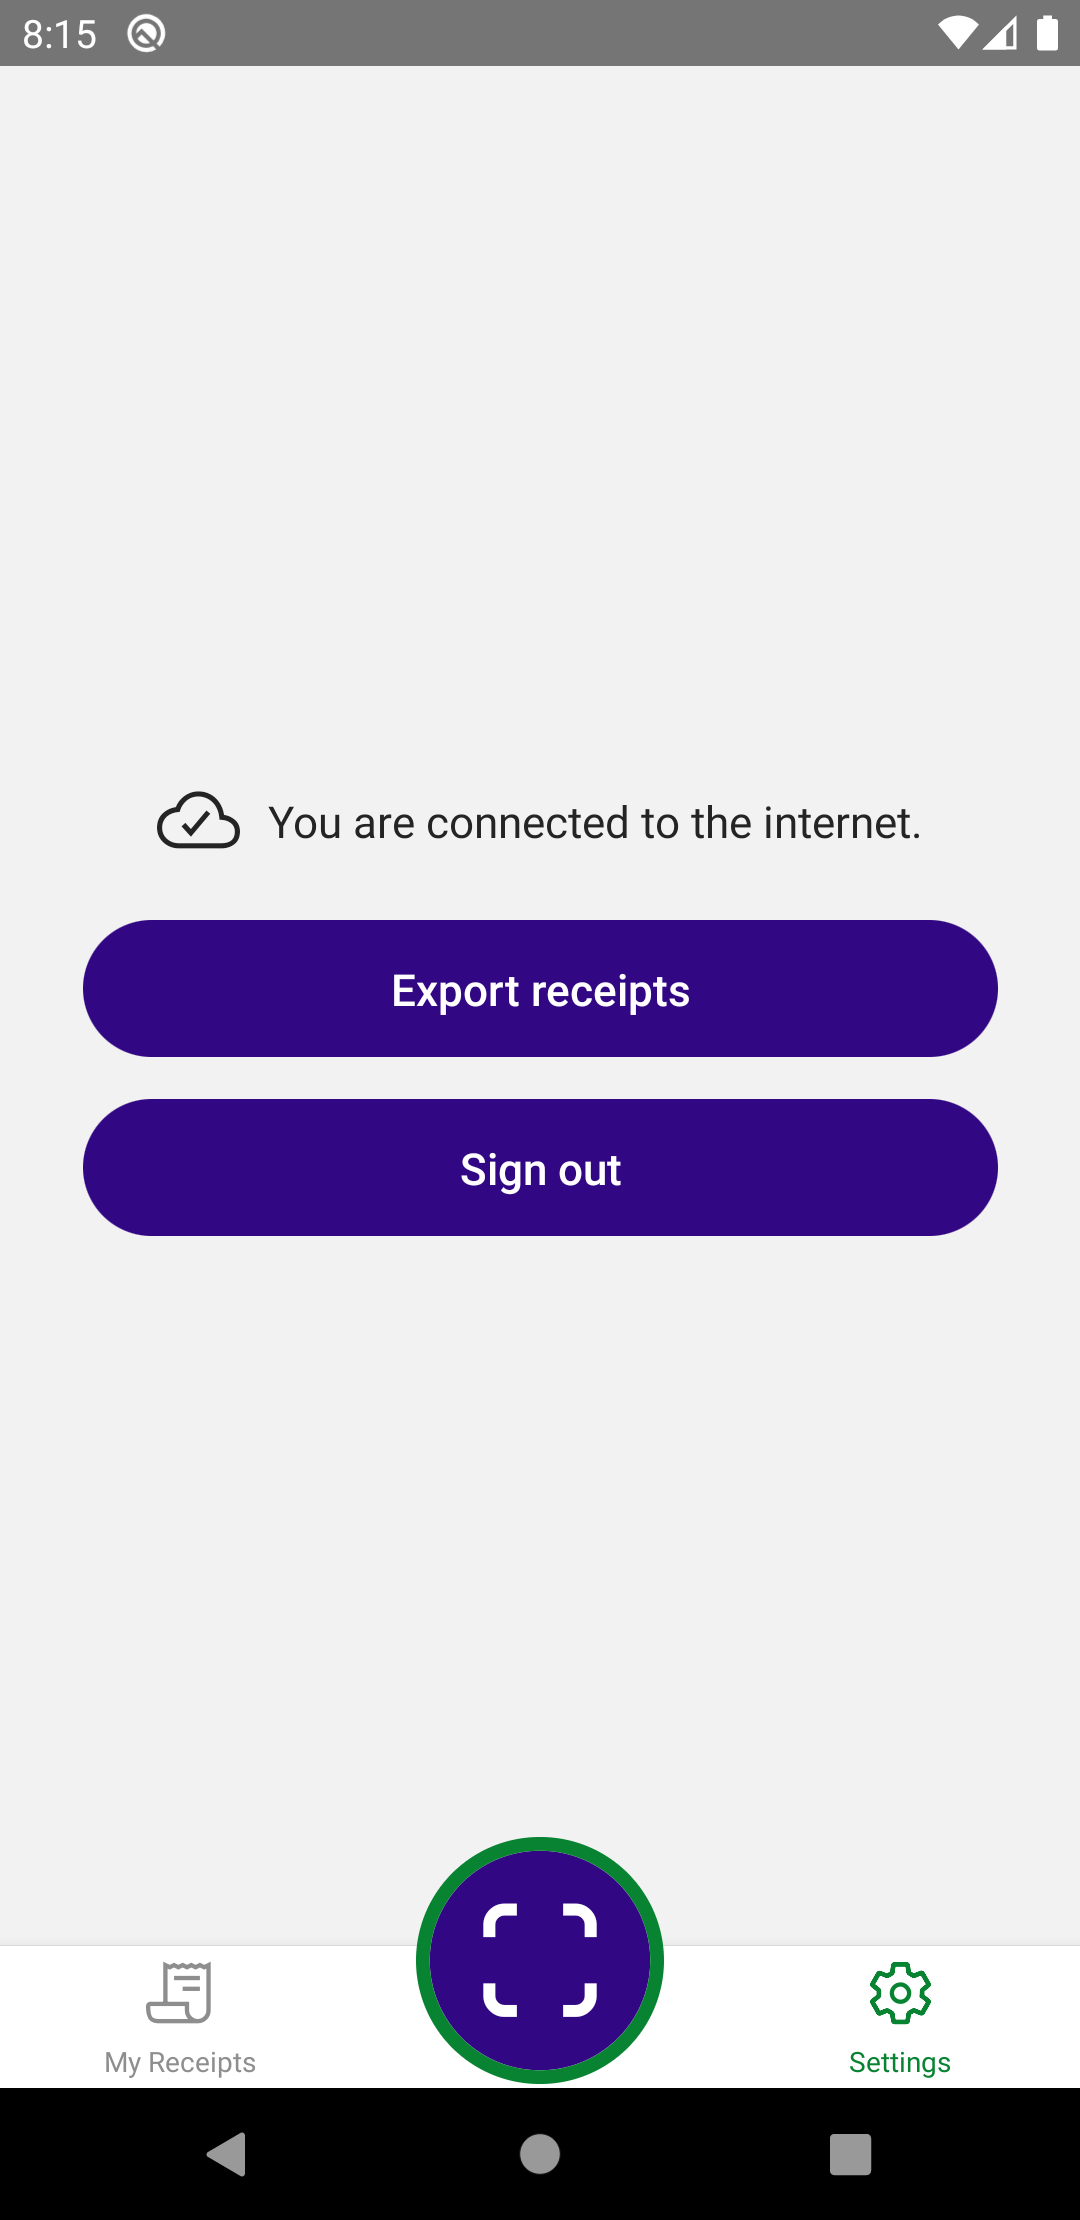
\includegraphics[width=0.5\textwidth]{figures/screens/android/light/settings_screen}
    \end{center}
    \caption{Settings screen with ``Sign out" ``Sign out'' button.}
    \label{fig:settings_screen}
\end{figure}

\chapter{Financial sustainability}
The Receipts Scanner uses paid third-party services, namely Microsoft Form Recognizer for OCR, Google Cloud Build, Google Container Registry and Google Cloud Run for deployment of Python API container and Google Firebase for document database and image storage. The Firebase Authentication is free.

It would be necessary to run the application for a period of time to figure out the usage statistics, such as the average number of receipts a user uploads. Since those statistics are not available yet, I will provide an estimate of the operational costs.

Let us assume that the application has \num{1000} active users, where each user makes one scan per day on average.
The price for Microsoft Form Recognizer is \$0.01 per scan \cite{FormRecognizerPricing}. This means the total cost of this service would be $\num{1000}\cdot30\cdot\$0.01 = \$300.00$.

The size of an uploaded image is around 500 KB, the processed image is smaller, around 100 KB large. The price of storing the textual data is negligible compared to other costs and would be lost in the approximations. Cloud Firestore is a very cheap storage \cite{CloudFirestorePricing} and its free tier provides storage for 1 GB, which is about \num{400000} average-sized receipts\footnote{The size of a stored receipt, \num{2500} KB, was computed using the \textit{firestore-size} library available at \url{https://github.com/alekslario/firestore-size}.}.

Whereas the number of scans is linearly proportional to the number of users, the numbers of stored receipts grows quadratically. It can be written recurrently as: 
\begin{equation}
r(n) = r(n-1) + cn
\end{equation}
or as a function of $n$:
\begin{equation}
r(n) = \frac{c}{2}n(n + 1)\text{,}
\end{equation}
where $n$ is a point in time (e.g. month) and $c$ is the number of receipts per user per chosen time period, in this case month. Since we assume one receipt per user per day, $c = 30$. A graph of this function is shown in Figure \ref{fig:receipts_by_users}

\begin{figure}
    \begin{center}
        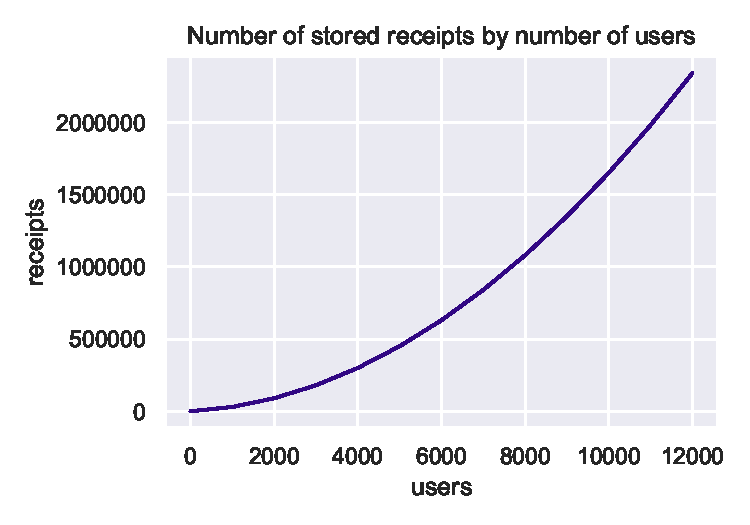
\includegraphics[width=0.7\textwidth]{figures/graphs/receipts_by_users}
    \end{center}
    \caption{Number of stored receipts by number of users}
    \label{fig:receipts_by_users}
\end{figure}

The images of receipts are stored on Google Cloud Storage. The price is \$0.026 per GB \cite{CloudStoragePricing}. For the first month, the cost would be $\num{1000}\cdot30\cdot(600\text{ KB} / 1\text{ GB})\cdot\$0.026 = \$0.468$.
For the second, assuming \num{1000} new users, it would be \$1.404.

The Google Container Registry is charged the same way as Google Cloud Storage \cite{ContainerRegistryPricing}, depending on the size of all stored containers. Only a few last containers need to be stored. Older containers can be deleted\footnote{Google provides an automated way of deleting old containers available at https://github.com/sethvargo/gcr-cleaner.}. This means that the price for stored containers will be fixed. The size of one Python API container is 2.7 GB. The price of storing 5 last containers would be $5\cdot2.7\cdot\$0.02 = \$0.27$ per month. 

Google Cloud Run provides autoscaling, which means that the number of provisioned instances depends on the number of incoming request. If a minimum number of instances is set to 0, the service goes idle each time the requests are not coming. The service is set up to use 2 CPUs and 6 GB of memory. For each receipt, one request is made to process the image and one to assign categories to items, therefore $\num{1000}\cdot30\cdot2 = \num{60000}$ requests per month. Assuming that each request comes after the previous ended and \num{1000} ms per request, the service will be used only for \num{120000} vCPU-seconds\footnote{vCPU-seconds are computed as $\textit{number of CPUs} \times \textit{time in seconds the service is running}$.}. This is included in the free plan. Memory consumption would be \num{480000} GiB-seconds\footnote{GiB-seconds are computed as $\textit{size in GiB} \times \textit{time in seconds the service is running}.$}, which slightly exceeds the free plan \cite{CloudRunPricing}, incurring \$0.3 of additional costs. 
If a minimum number of instances was set to 1 in order to prevent a cold-start, the cost would be \$66.00 per month.

Building a container using Google Cloud Build takes approximately 9 minutes. The price is \$0.016 per build-minute \cite{CloudBuildPricing}. Assuming 3 builds per day due to code changes pushed to master branch, the cost per month is $3\cdot9\cdot\$0.016\cdot30 = \$12.96$.

The total operational cost per month with \num{1000} users would be \$314.00, i.e \$0.314 per user.
From Figure \ref{fig:operational_costs} is apparent that most of these costs are due to the OCR service. This is why also other application offer this feature only after paying a fee. Smart Receipts charges \$0.10 per one OCR scan.

\begin{figure}
    \begin{center}
        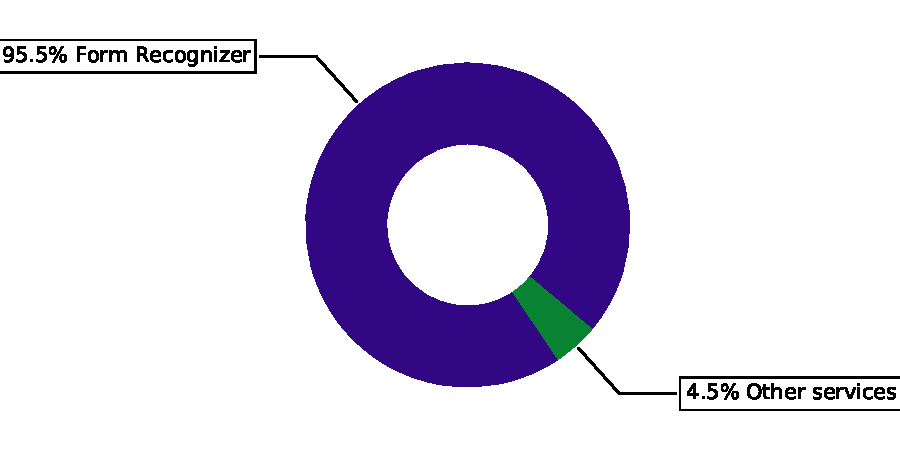
\includegraphics[width=1\textwidth]{figures/graphs/operational_costs}
    \end{center}
    \caption{Operational costs of using Form Recognizer compared to other services}
    \label{fig:operational_costs}
\end{figure}

The Receipts Scanner would therefore need to have its own OCR service or become monetized. I think that in-app advertising, such as AdMob\footnote{Mobile app monetization from Google}, would not generate enough revenue. A subscription-based model would be in my opinion a more viable option. The third option would be a combination of the two previous approaches -- a limited number of scans and visible advertisement for non-subscribed users and an unlimited number of scans and removed advertisement for the subscribed ones.


\chapter{Downsides of current OCR solution}
price
works only with english receipts, would need to be retrained

The goal of my thesis is to develop a mobile application, that would allow a user to take a photo of a receipt and save it to their private receipt database. TODO taky možnost nahrát ze zařízení. The application should recognize information on the receipt, such as merchant, individual items together with their prices and the overall price of the purchase. TODO co všechno pozná. It would then use this information to prefill TODO později rozebrat že pomocí OCR, definovat OCR; the form fields associated with the receipt, that could be then further edited. The saved receipts could be then easily searched and used when complaining or returning goods.
The application would also have a desktop version, that would allow only the search capabilities, without an option to scan new receipts.

I have created such application and named it Receipts Scanner. Apart from the features mentioned above, it can also categorize items and visually convey the item category by associating an emoji with it. It also stores the photo of the receipt in two formats. The first is the original photo and the second is an augmented photo that is easier to read. TODO porovnat, že se skutečně lépe čte. Průzkum? Tabulka. 20 lidí, 10 účtenek.

\chapter{Item categorization}
In order to make the application more visually attractive and to improve the user experience, each item on the receipt is assigned an emoji. The emoji is chosen base on the words that appear in the item name. If the user is not content with the automatically assigned category, they can remove it in the receipt edit form.

When a user adds a new receipt, the items on the receipt are sent to the Python API \texttt{/category} endpoint. The service contains a dictionary of category names as keys and emojis as values. Each item name is compared to all dictionary keys by using method \texttt{most\_similar\_to\_given} and the key that is most similar to the item name is returned, together with the emoji.

The method \texttt{most\_similar\_to\_given} is provided by the Magnitude library\cite{patel-etal-2018-magnitude}. Magnitude is a tool for utilizing and processing word embeddings. Word embeddings are typically real-valued vectors that encode the meaning of a word, such that the vectors that are close in the vector space are similar in their meaning \cite{Jurafsky2020}. Magnitude is a faster and memory efficient alternative to tools like Gensim\footnote{\url{https://radimrehurek.com/gensim/}}. 

It uses its own vector storage file format \texttt{.magnitude}.
Popular embedding models such as Google's word2vec, Stanford's GloVe and Facebook's fastText have been pre-converted to the \texttt{.magnitude} format for immediate download and usage\footnote{Pre-converted models for immediate download: \url{https://github.com/plasticityai/magnitude\#pre-converted-magnitude-formats-of-popular-embeddings-models}}. Furthermore, each word embeddings model is available in three variants -- light, medium and heavy. The difference is that medium and heavy models have advanced support for out-of-vocabulary keys\footnote{Words that do not appear in the model's vocabulary.}. The heavy model also features faster approximate k-nearest neighbors. 

Magnitude implements functions for looking up
vector representations for misspelled or out-of-vocabulary words. This means it can handle abbreviations, which often appear on receipts, and whole sentences reasonably well.

The interface of the library is agnostic to the underlying model.
In Receipt Scanner, the fastText model is used – in particular its medium variant, as only the exact similarity search is performed, so there is no need for faster approximate k-NN. The light variant handles item names that contain multiple words poorly.

Another constraint for choosing the model was its size. Google Cloud Run, which is a cloud service where the model is running, does not allow containers larger than 8 GB. The Google's medium word2vec model is 4.9 GB large, as compared to fastText, which is only 1.6 GB large. The container with word2vec did not fit into the 8 GB limit.

The used fastText model was pretrained on over 16 billion words from Wikipedia 2017, Statmt.org news and UMBC news \cite{mikolov2018advances}. It contains only English word vectors, but fastText provides also models for other languages \footnote{Word vectors for 157 languages: \url{https://fasttext.cc/docs/en/crawl-vectors.html}}, which could be converted using the Magnitude converter\footnote{Magnitude converter: \url{https://github.com/plasticityai/magnitude\#file-format-and-converter}} and used in a localized Receipts Scanner, e.g. with a support for Czech language.

Figure \ref{fig:models_comparison} shows results from various word embeddings models. First two columns are generated by Google's word2vec, which was trained on 1 billion words from Google News. The third column is the mentioned fastText. The fourth column is fastText with subwords information. In subwords model, each word is represented as a bag of character \textit{n}-grams. Taking the
word \textit{where} and $n = 3$ as an example, it will be
represented by the character \textit{n}-grams:
\[
<\text{wh, whe, her, ere, re}>
\]
and the special sequence $<\text{where}>$. $<$ and $>$ are special boundary symbols. \cite{bojanowski-etal-2017-enriching}

The results show that the case matters, e.i. "CHUPA LOLLIPOPS" vs "Chupa lollipops", and how more concrete terms are mapped to more general terms, e.i. "salmon" and "cola" are categorized as "fish" and "cold beverage" respectively.

\begin{figure}
    \begin{center}
        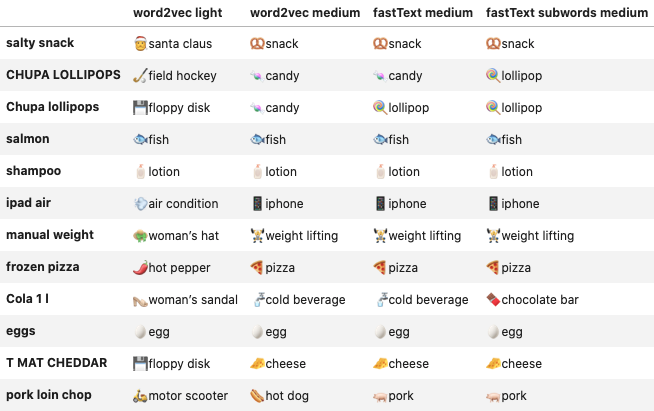
\includegraphics[width=1\textwidth]{figures/tables/model_comparison}
    \end{center}
    \caption{Comparison of pretrained word embeddings models.}
    \label{fig:models_comparison}
\end{figure}

\chapter{Image processing}
The image processing happens independently of the OCR. It does not have any effect on the text recognition and information extraction, because the \textit{original} image is sent to the Form Recognizer API. The purpose of image processing happening in the Receipts Scanner is to provide a cleaner preview of the receipt. The result is a cropped picture with black text on a white background. The whole process consists of the following steps:

\textbf{1) Loading image:} The image is loaded in a grayscale.

\paragraph{2) Noise removal:} Gaussian blur is applied to reduce the Gaussian noise in the image. It is the most common type of noise in an image \cite{OCRCNN}. The blur is achieved by convolving the image with a Gaussian function.

\begin{equation}
G(x,y) = \frac{1}{2\pi\sigma^2}e^{-\frac{x^2+y^2}{2\sigma^2}}\text{,}
\end{equation}

where $x$ and $y$ are the distances from the origin in the horizontal and vertical axis, respectively. $\sigma$ is the standard deviation of the Gaussian distribution. \cite{OCRCNN}

A result of applying Gaussian blur is shown in Figure \ref{fig:gaussian_blur}.

\begin{figure}
    \centering
    \begin{subfigure}[t]{0.5\textwidth}
      \centering
      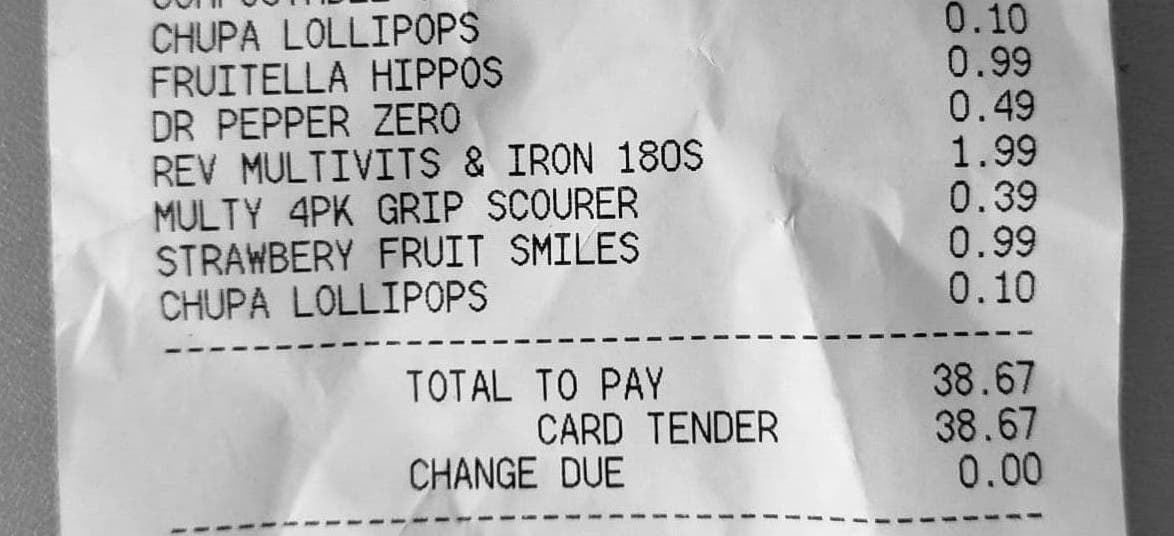
\includegraphics[width=0.95\textwidth]{figures/image_processing/before_blur}
      \caption{Before Gaussian blur.}
    \end{subfigure}
    \begin{subfigure}[t]{0.5\textwidth}
      \centering
      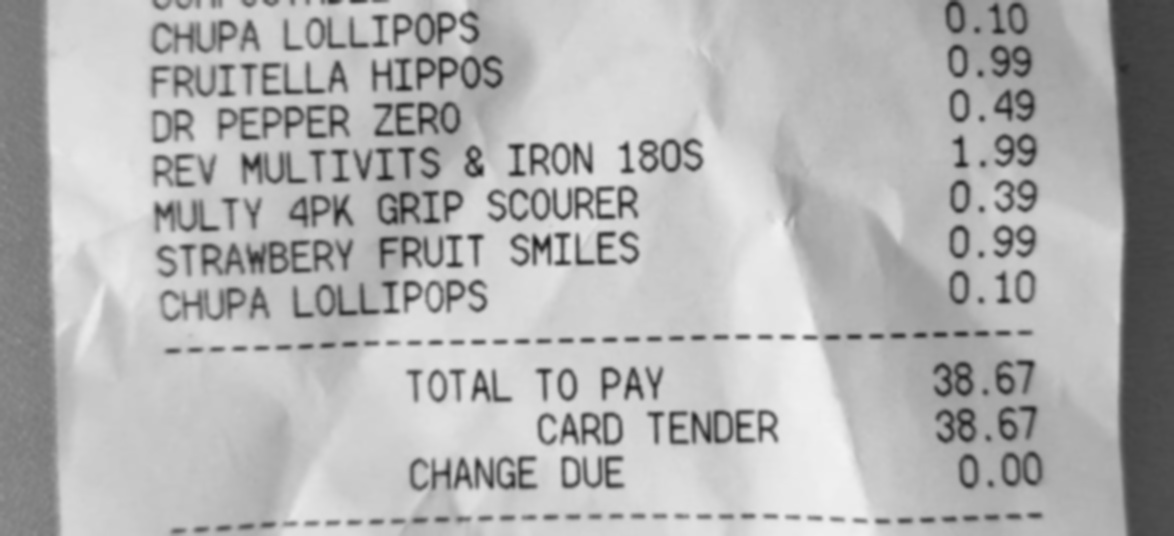
\includegraphics[width=0.95\textwidth]{figures/image_processing/after_blur}
      \caption{After Gaussian blur.}
    \end{subfigure}
    \caption{Comparison of an image before and after Gaussian blur has been applied.}
    \label{fig:gaussian_blur}
\end{figure}

\paragraph{3) Binary thresholding:} For better accuracy on detection of the edges and contours, it is beneficial to convert the images to binary images. Binary tresholding sets pixel value to the maximum value, which is usually 255 (white), if its value is greater than the threshold, otherwise the pixel value is set to 0 (black).

\begin{equation}
\label{eqn:binary_tresholding}
dst(x,y) = \begin{cases}
            \texttt{maxval} & \text{if }src(x,y) > \texttt{thresh}\\
                0 & \text{otherwise}
          \end{cases}
\end{equation}

In equation \ref{eqn:binary_tresholding} $src(x,y)$ is a value of a source pixel on coordinates $x$ and $y$ and $dst(x,y)$ is a value of destination, i.e. resulting pixel, on coordinates $x$ and $y$.

The threshold value can either be fixed, e.g. 127, or it can be computed from the image. Finding the right value for the fixed thresholding is difficult and each image might have a different optimal threshold value. 

Otsu's thresholding calculates the threshold value dynamically from the histogram of each image, such that the found threshold maximizes the between-class variance \cite{gonzalez08}. Classes are black and white pixels.

Figure \ref{fig:binary_threshold} shows a result of applying fixed binarization with threshold value of 127. The edges of a receipt would not be correctly recognized, because the value is too small for this photo of a receipt. 

Figure \ref{fig:otsu_threshold} shows a result of applying Otsu's thresholding, which automatically found a threshold value of 151. The edges are clearly visible.

\begin{figure}
    \centering
    \begin{subfigure}[t]{0.5\textwidth}
      \centering
      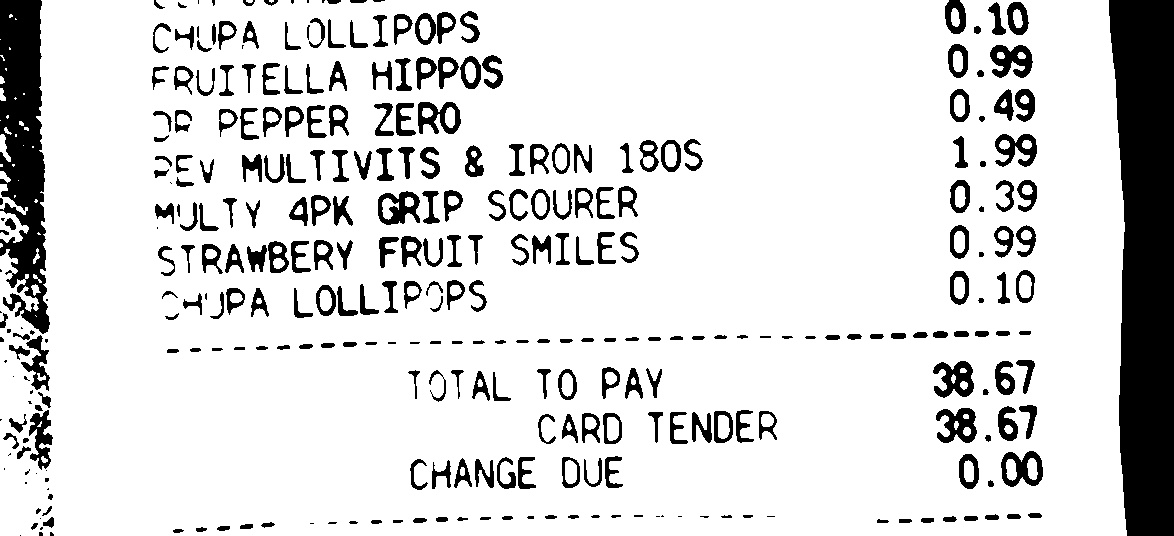
\includegraphics[width=0.95\textwidth]{figures/image_processing/binary_threshold}
      \caption{Binarized image with fixed threshold of 127.}
      \label{fig:binary_threshold}
    \end{subfigure}
    \begin{subfigure}[t]{0.5\textwidth}
      \centering
      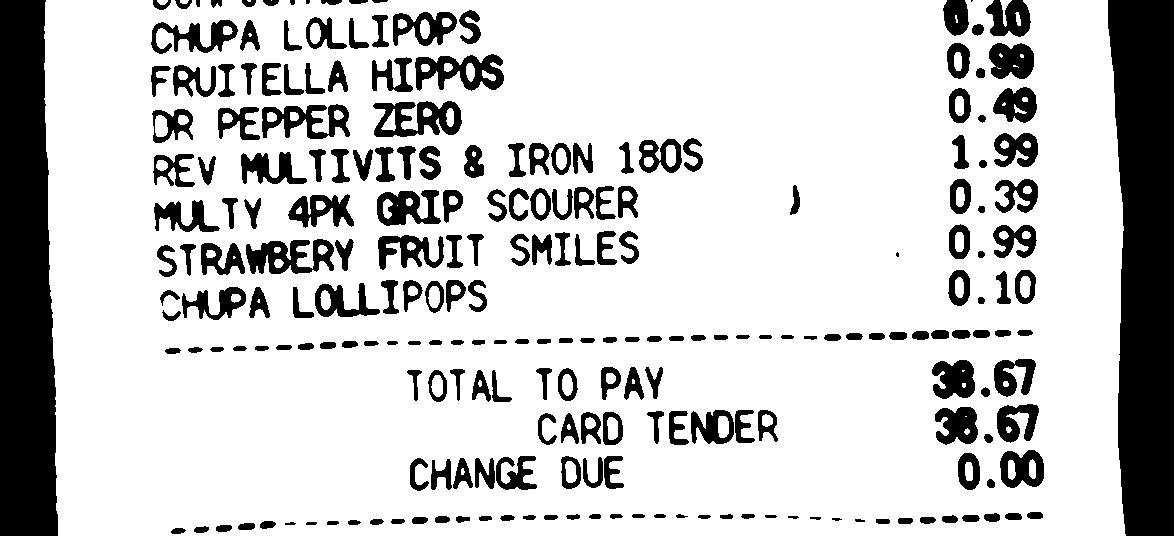
\includegraphics[width=0.95\textwidth]{figures/image_processing/otsu_threshold}
      \caption{Binarized image with threshold of 151 found by Otsu's method.}
      \label{fig:otsu_threshold}
    \end{subfigure}
    \caption{Comparison of a fixed and Otsu's thresholding.}
    \label{fig:threshold_comparison}
\end{figure}

\paragraph{4) Dilation:} In order to determine edges of the receipt more easily, the image is dilated. Dilation increases the size of the grid lines.

Before performing dilation, the image has to be inverted, otherwise an opposite effect, erosion, would be achieved. It is necessary to invert the image back before contour detection, which is described in the next step. 

A kernel slides through the image, the same way as in 2D convolution. A pixel will be considered white if at least one pixel in the original image under the kernel is white.

A result of applying dilation is shown in Figure \ref{fig:dilation}.

\begin{figure}
    \centering
    \begin{subfigure}[t]{0.5\textwidth}
      \centering
      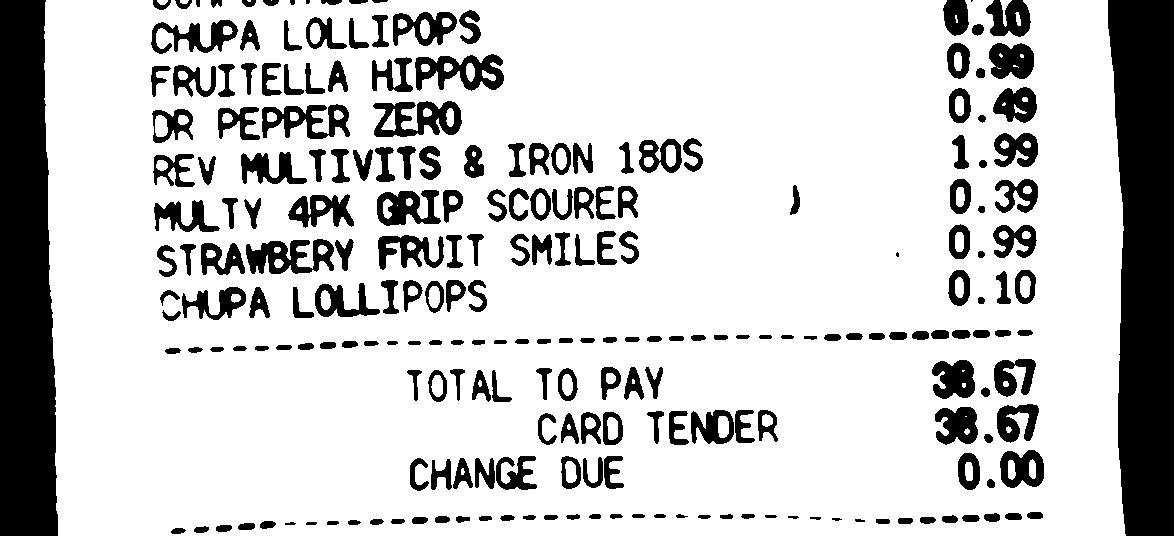
\includegraphics[width=0.95\textwidth]{figures/image_processing/before_dilation}
      \caption{Before dilation.}
    \end{subfigure}
    \begin{subfigure}[t]{0.5\textwidth}
      \centering
      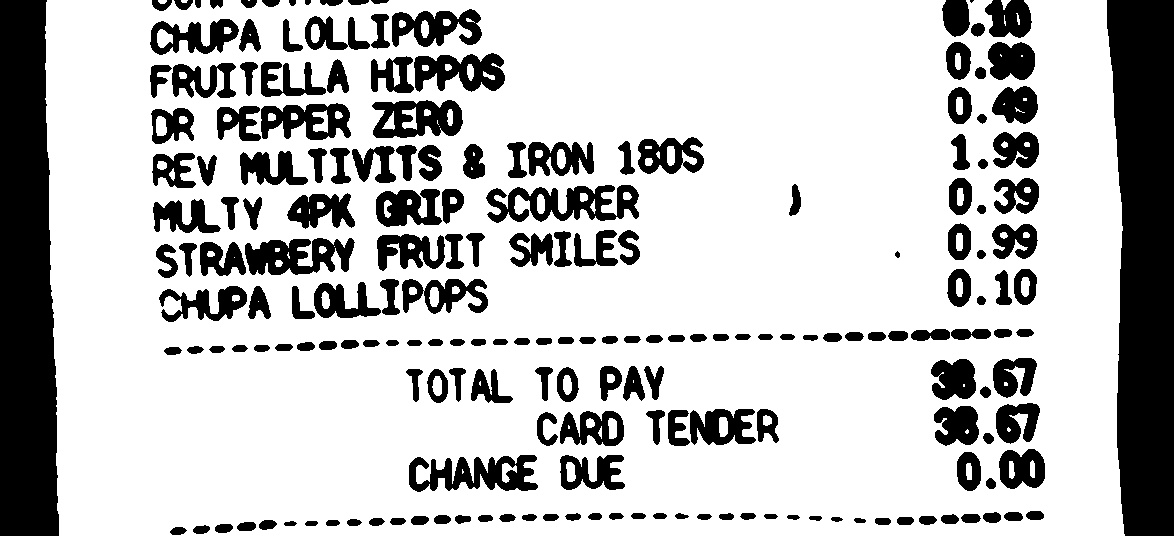
\includegraphics[width=0.95\textwidth]{figures/image_processing/after_dilation}
      \caption{After dilation.}
    \end{subfigure}
    \caption{Comparison of an image before and after dilation has been applied.}
    \label{fig:dilation}
\end{figure}

\paragraph{5) Finding the corners of a receipt:} As a next step, all external contours in the image are found. Contour is a curve joining points of the same color and intensity. The contour with the largest area is most probably the contour of a receipt. Four points that represent the corners of the receipt are then found in the contour and returned. A result of this step is visualized in Figure \ref{fig:points_and_edges}.

However, if the area of the contour is smaller than 30\% of the overall image, the next step, \textit{Cropping and warping}, will be skipped.

\begin{figure}
    \begin{center}
        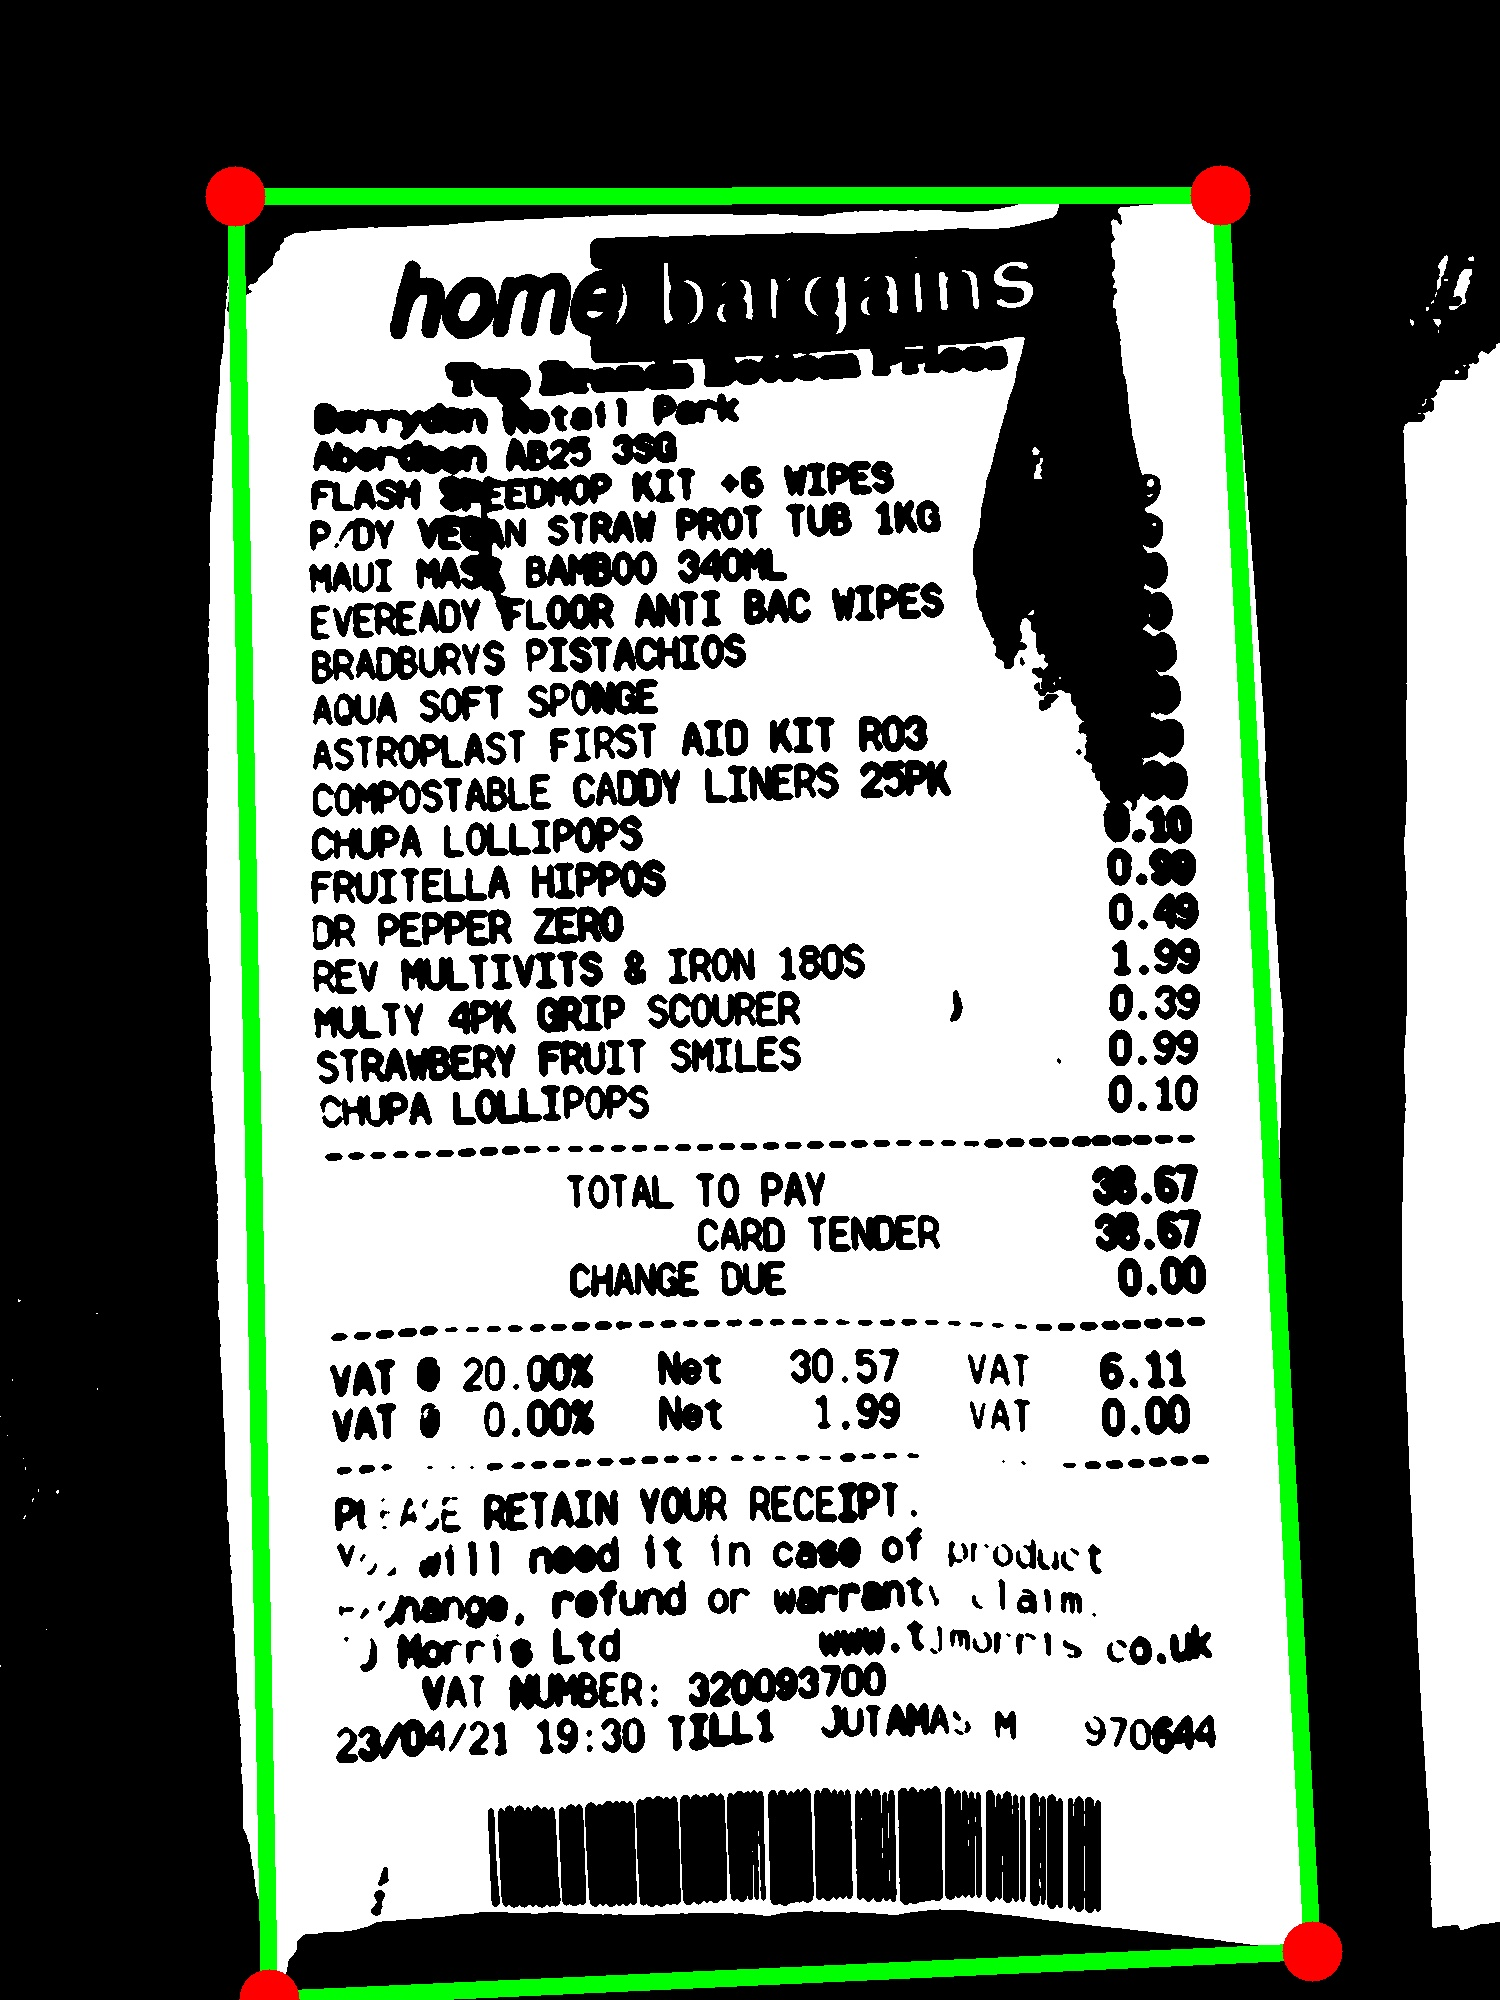
\includegraphics[width=0.5\textwidth]{figures/image_processing/points_and_edges}
    \end{center}
    \caption{Binarized photo with recognized corners.}
    \label{fig:points_and_edges}
\end{figure}

\paragraph{6) Preparing underlying picture} The previous steps were used to find the corners of a receipt. Although Otsu's thresholding made the edges of the white receipt clearly distinguishable from the dark background, the text of the receipt became unreadable. 

A different scenario would be for receipt scans. Since scans usually do not have any background, Otsu's thresholding results in a larger contrast between the paper and text as opposed to a contrast between the paper and the background.

For receipt photos, adaptive thresholding is a better choice. This is also caused by the presence of shades in the photos, which are not present in scans.

With adaptive thresholding, the threshold value for each pixel is based on a small region around it. This method gives better results for images with varying illumination. \cite{opencvtresholding}

OpenCV library provides two methods of computing the adaptive threshold. It can be computed as the mean of the neighbourhood area minus a constant $C$ or as a Gaussian-weighted sum of the neighbourhood values minus the constant $C$. Empirically, Gaussian method with $C = 2$ produced the best results.

Before the adaptive thresholding is applied, the original image is blurred using Gaussian blur. This improves the result significantly as can be seen in Figure \ref{fig:adaptive_thresholding}.

\begin{figure}
    \centering
    \begin{subfigure}[t]{0.5\textwidth}
      \centering
      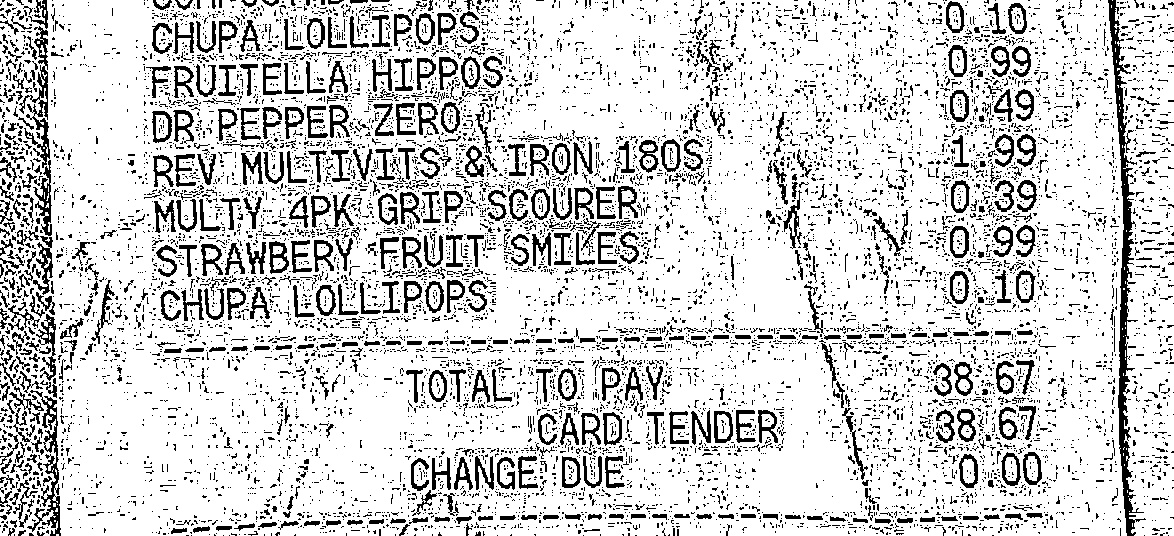
\includegraphics[width=0.95\textwidth]{figures/image_processing/adaptive_thresholding_no_blur}
      \caption{Adaptive thresholding without Gaussian blur.}
    \end{subfigure}
    \begin{subfigure}[t]{0.5\textwidth}
      \centering
      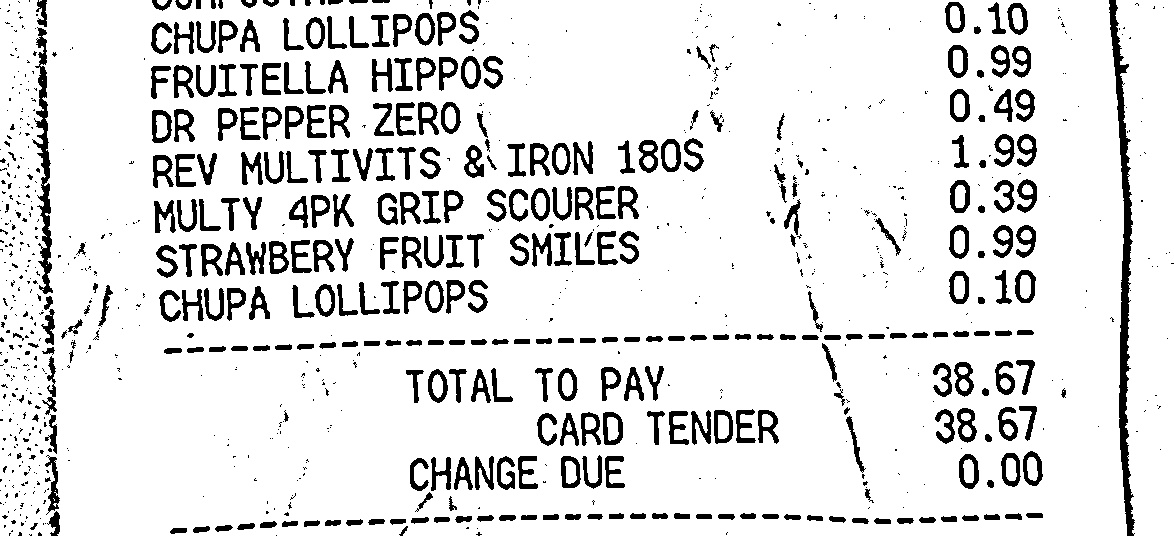
\includegraphics[width=0.95\textwidth]{figures/image_processing/adaptive_thresholding}
      \caption{Adaptive thresholding after Gaussian blur.}
    \end{subfigure}
    \caption{Comparison of an adaptive thresholding with and without Gaussian blur being applied first.}
    \label{fig:adaptive_thresholding}
\end{figure}

\paragraph{7) Cropping and warping:} Lastly, a perspective transformation (warping) is applied on the underlying photo produced by the previous step.
The found quadrilateral, represented by four corners, is warped into a rectangle of a similar size. This step also crops the receipt from the background. 

A comparison of the original image and the final processed image is shown in Figure \ref{fig:original_vs_processed}. The processed image is cropped and warped.

\begin{figure}
    \centering
    \begin{subfigure}[t]{0.5\textwidth}
      \centering
      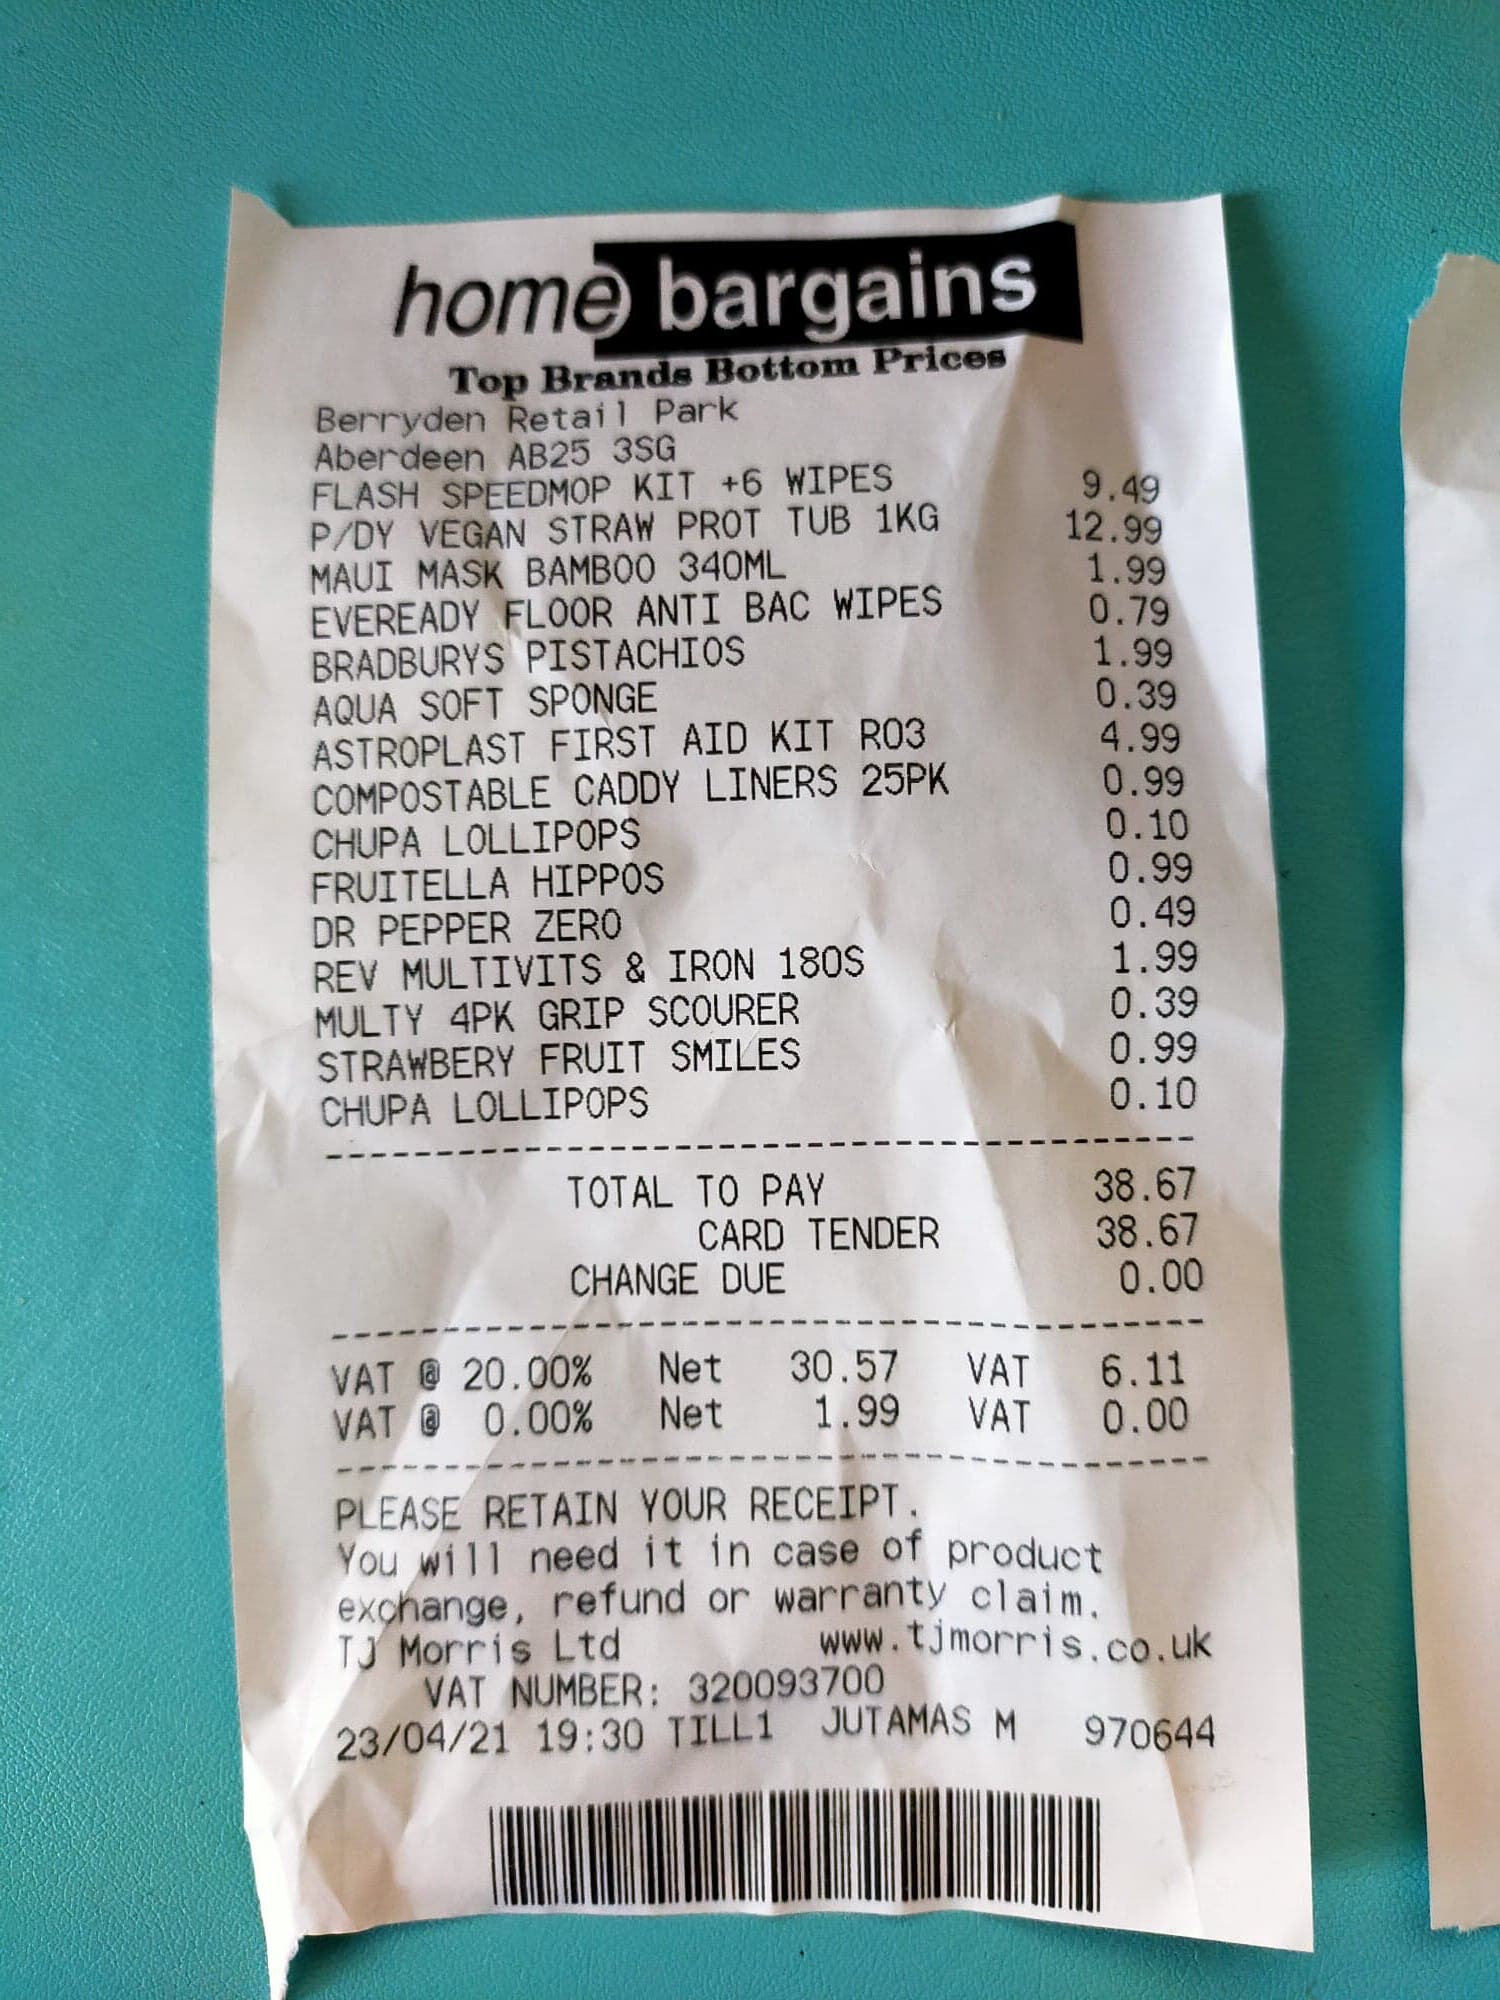
\includegraphics[width=0.95\textwidth]{figures/image_processing/original_image}
      \caption{Original image.}
    \end{subfigure}
    \begin{subfigure}[t]{0.5\textwidth}
      \centering
      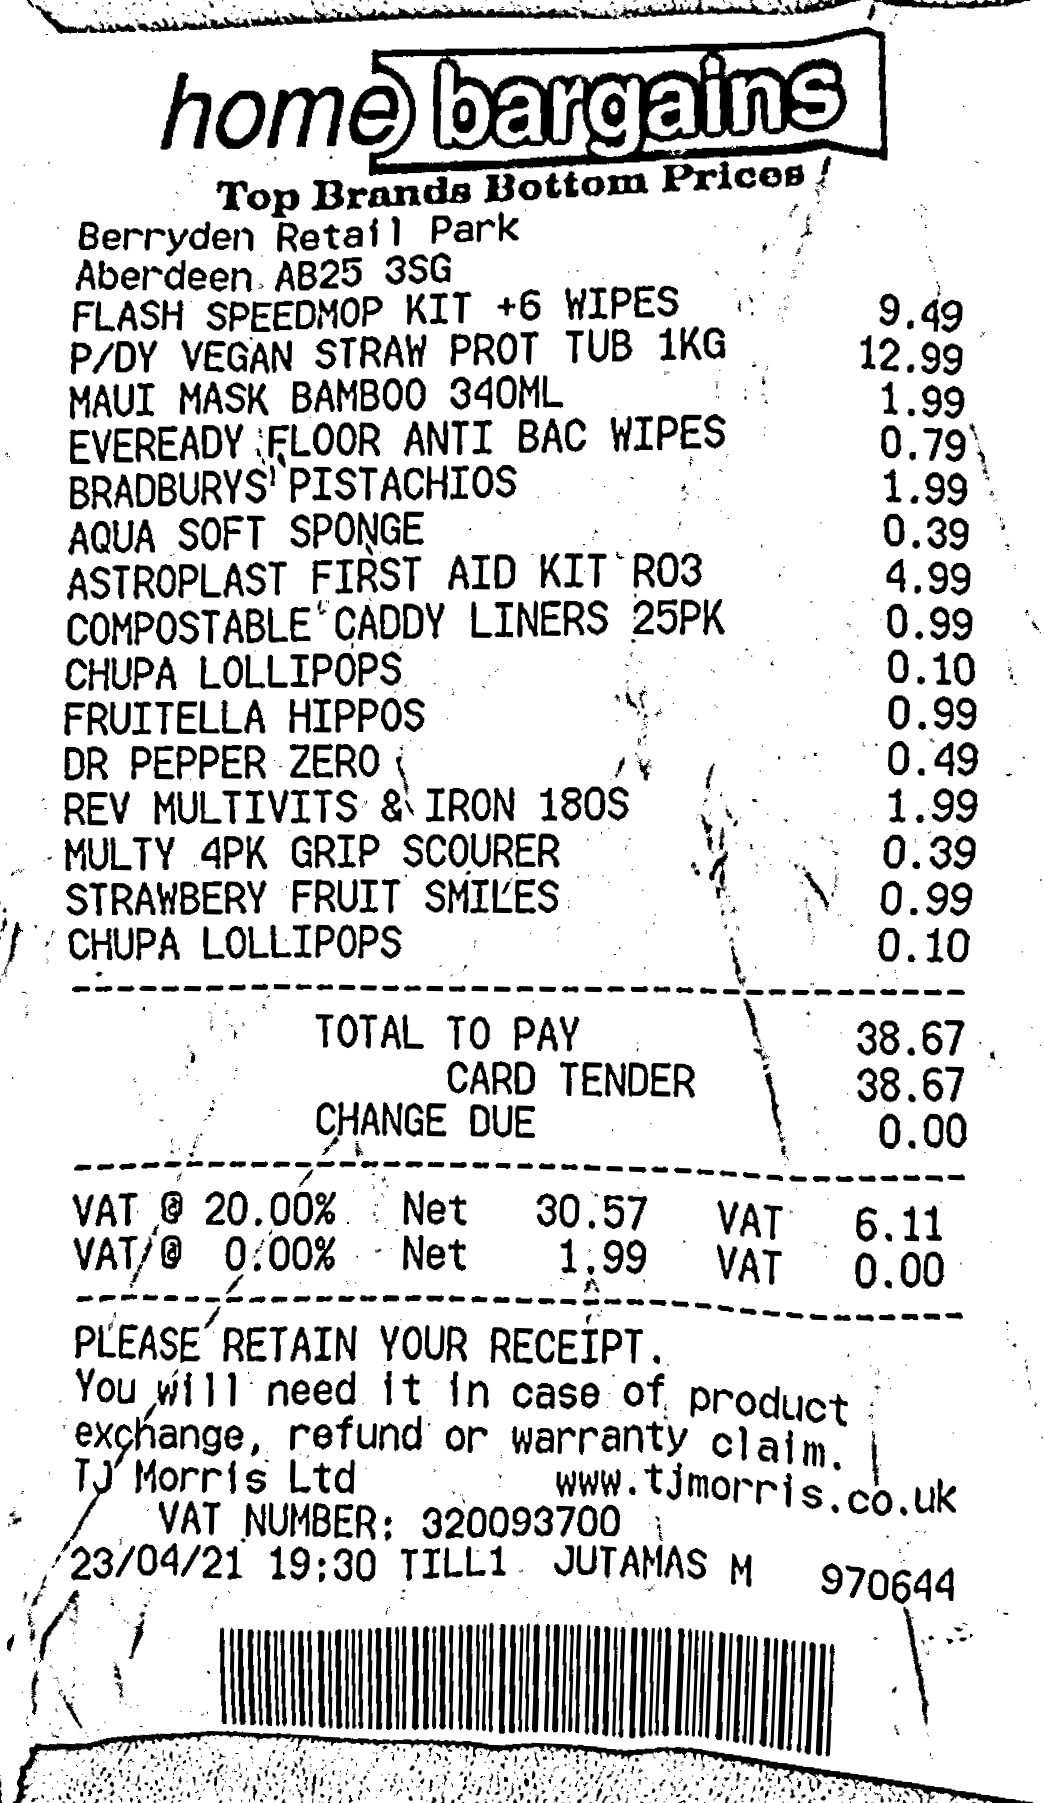
\includegraphics[width=0.95\textwidth]{figures/image_processing/processed_image}
      \caption{A processed image after adaptive binarization and perspective transformation.}
    \end{subfigure}
    \caption{Comparison of a fixed and Otsu's thresholding.}
    \label{fig:original_vs_processed}
\end{figure}

% Perspective transformation transforms the source image using a transformation matrix $M$:
% \begin{equation}
% dst(x,y) = src\left(\frac{M_{11}x+M_{12}y+M_{13}}{M_{31}x+M_{32}y+M_{33}},\frac{M_{21}x+M_{22}y+M_{23}}{M_{31}x+M_{32}y+M_{33}}\right)\text{.}
% \end{equation}

% $M$ is a $3\times3$ transformation matrix, computed as follows:


\chapter{Evaluation}
The application has not been been given to real users yet. Therefore there is no available feedback concerning usability, performance and the overall user experience.

The Form Recognizer API used for OCR and data extraction from an image is a third party service and as such measuring its performance would provide little value compared to the rest of the thesis. It would become more important if the current data extraction was not sufficient, which would be best found by users in practise. 

Quantifying how well Form Recognizer extracts the data from the photo would require a labeled set of receipts. One such set is available as part of the ICDAR2019 Competition on Scanned Receipt OCR
and Information Extraction \cite{ICDAR2019}. It provides \num{1000} labeled receipt scans\footnote{A corrected set of the original images is available on GitHub: \url{https://github.com/zzzDavid/ICDAR-2019-SROIE}.} as well as an evaluation technique. However, the labels from this dataset contain only \textit{company}, \textit{date}, \textit{address} and \textit{total}. Form Recognizer is able to recognize other information, such as phone number and individual items, too. Furthermore, the main use case in Receipts Scanner is recognition of photographed receipts, not receipt scans. Therefore a different dataset would be needed.

To evaluate the performance of item categorization and image processing, a questionnaire has been given to 28 people. It consists of two parts.

\subsection{Emojis}
The purpose of this section is to evaluate how accurately the emoji chosen by the categorization service inside Python API fits to the text. The text is the name of a receipt item recognized by Form Recognizer, consisting of one or more words.

70 items have been selected from the data extracted by Form Recognizer on various receipts, excluding items that were incorrectly classified as a receipt item. Duplicates and similar items have not been included in this set either.

For each item and its assigned emoji, the task was to choose whether the emoji is \textit{Not accurate}, \textit{Mildly accurate} or \textit{Accurate}.

\begin{figure}
    \begin{center}
        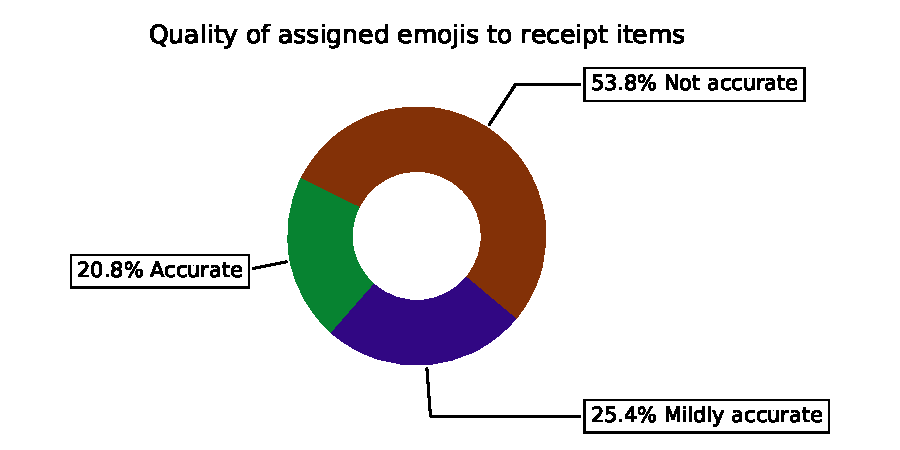
\includegraphics[width=0.7\textwidth]{figures/graphs/quality_of_emojis}
    \end{center}
    \caption{fdsfsd}
    \label{fig:quality_of_emojis}
\end{figure}

\subsection{Images}

\begin{figure}
    \begin{center}
        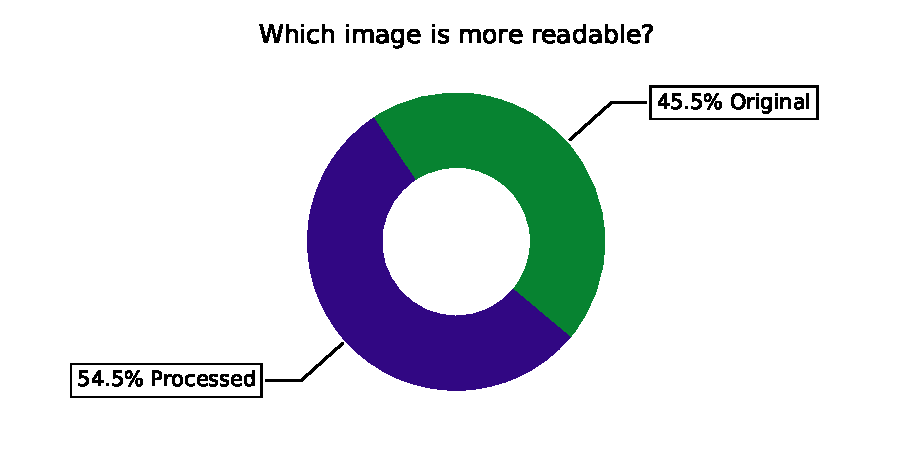
\includegraphics[width=0.7\textwidth]{figures/graphs/which_image_is_more_readable}
    \end{center}
    \caption{fdsfsd}
    \label{fig:which_image_is_more_readable}
\end{figure}


Receipts used in the survey are a combination of receipts collected among friends and ExpressExpense \cite{ExpressExpense2019} dataset.

\chapter{Emoji}
When working with a version control system \footnote{A software for tracking changes in files, for example Git.}, it is a good practise to indicate a type of a commit. This can be done either verbally or using an emoji.
Using emojis in commit messages provides an easy way of identifying the purpose or intention of a commit. In Receipts Scanner repository, the notation in Figure \ref{fig:emoji_commits} has been used. It is loosely based on Gitmoji \footnote{Gitmoji is an initiative to standardize and explain the use of emojis on GitHub commit messages. See \url{https://gitmoji.dev/}}. The Figure shows a Unicode representation of an emoji and its meaning.
    \begin{figure}
        \begin{center}
            \includegraphics[width=\textwidth]{figures/other/Emoji_commits}
        \end{center}
        \caption{Meaning of emojis in commit messages.}
        \label{fig:emoji_commits}
    \end{figure}


\chapter{Python API}
The Python API serves two purposes: to process an image of a receipt and to categorize receipt items.

It provides three endpoints \footnote{The detailed documentation of endpoints is available here: \url{https://documenter.getpostman.com/view/9355808/TzJsfdUK}}:

\begin{itemize}
    \item \texttt{GET /} -- Returns a health check string. Used to make sure that the service is running.
    
    \item \texttt{POST /category} -- Expects a JSON containing an item name, possibly consisting of multiple words. It returns a category of that item.
    
    \item \texttt{POST /process-image} -- Expects a form-data containing an image. It returns the processed version of that image.
\end{itemize}

\section{Deployment}
The Python API is a Flask\footnote{See \url{https://flask.palletsprojects.com/en/1.1.x/}.} server. 
It is deployed after each push to the master branch.
First, a Docker image that contains the source files, external dependencies and the Magnitude word embeddings model is built using Google Cloud Build. The built image is saved into Google Container Registry. Google Cloud Run then start a container from that image.
It the image was not built successfully or the service failed to start, the previously deployed service will stay available.

API tests are run during the CI pipeline after the new service is deployed.  

\chapter{Storage}
The Receipt Scanner needs to two kinds of data: textual data, which are data about the receipts and the users' credentials, and the receipt images. 

\section{Textual data}
For textual receipt information, document-oriented databases are a perfect fit, because they make it easy to store data in the same format and shape as they are used in the application. 

The document-oriented database is a type of NoSQL\footnote{NoSQL database is a database that does not employ the relational model of data \cite{DigitalOcean2019}} database that stores data in the form of documents. All data of a given object (for example receipt) can be stored in one document. The documents are stored mostly in JSON\footnote{JavaScript Object Notation}, BSON\footnote{Binary JSON;}, XML\footnote{Extensible Markup Language} or YAML\footnote{YAML is a human-readable data-serialization language.} format. Unlike SQL databases, document-orient databases do not have a schema and are therefore more flexible. 
The documents are stored in collections. Documents can also contain subcollections of documents.
Two very popular document-oriented databases are MongoDB\footnote{See \url{https://www.mongodb.com/}} and Google Firestore\footnote{See \url{https://firebase.google.com/products/firestore}}. MongoDB uses BSON to store documents, Firestore uses JSON. Both databases support data types such as strings, numbers, arrays and timestamps. 
% https://www.tutorialspoint.com/mongodb/mongodb_datatype.htm
Although document-oriented databases do not have a schema, it is very useful to have a fixed data model, so that the shape of the stored data is predictable. 
The data model for Receipts Scanner is shown in Figure \ref{fig:data_model_firestore}. It shows how the data are structured into two collections, \texttt{Users} and \texttt{Receipts}. Because all user data are child nodes of a given user document, it is easy to restrict access to other documents based on the path to that document.

Although the item forms a separate entity, it is not a document, but only an object in the array of items of the receipt.

Other notable fields are \texttt{urlOriginal} and \texttt{urlProcessed}, which specify the URL address of the original receipt photo and a processed photo, respectively. 

    \begin{figure}
        \begin{center}
            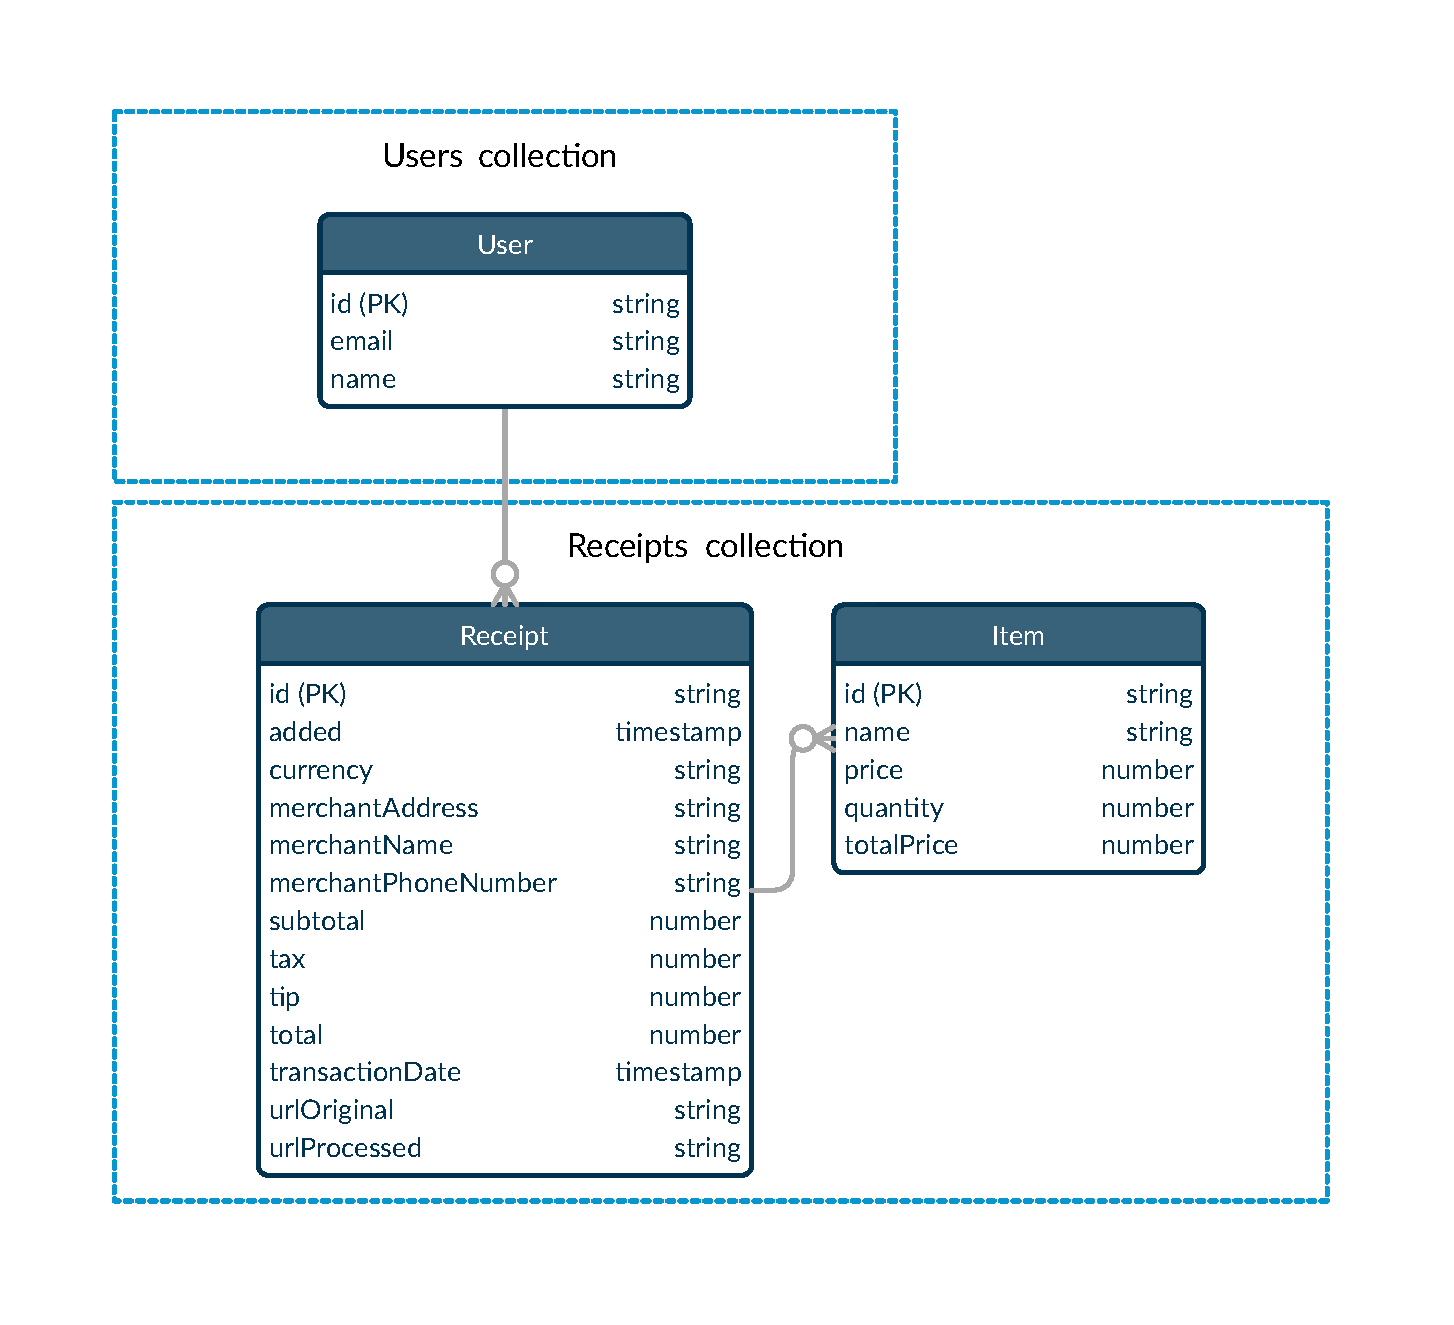
\includegraphics[width=\textwidth]{figures/other/data_model_firestore}
        \end{center}
        \caption{Data model of Receipts Scanner}
        \label{fig:data_model_firestore}
    \end{figure}

\section{Image data}
Although storing images directly in the document-oriented database would be possible \footnote{In MongoDB, it is possible to store BSON documents up to 16 MB. Larger files can be split into parts of 255 kB using GridFS \cite{GridFS}}, this solution is not optimal.

For receipt images, the most cost-effective storage is an object storage. An object storage is a storage optimized for storing BLOBs (Binary Large OBjects). BLOB is a collection of binary data stored as a single entity. It can be for example an image, audio or video. 

The images are stored inside \texttt{Users/<user\_id>/Receipts/} directory. This folder structure enables restricting access to images based on the value of \texttt{<user\_id>}.

I have chosen Google Firestore to store the textual data and Google Storage to store the photos of receipts. These two cloud-based services are available under a platform called Firebase. The Firebase platform provides also the authentication and analytics services to Receipts Scanner.

Firebase is supported on iOS, Android and Web. An unofficial library called React Native Firebase\footnote{\url{https://rnfirebase.io/}} provides the same services on React Native for Android and iOS. However, it does not support React Native Windows. Therefore Receipts Scanner uses Firebase for Web on Windows and React Native Firebase on Android. To be able to write the same code that could be run both on Android and Windows, an adapter `firebase.ts` was created. It imports both libraries and based on the platform the application is currently running on exports the right objects. Rest of the code that needs to work with Firebase imports the objects from `firebase.ts` instead of importing either from Firebase for Web or React Native Firebase directly.

In theory, the Receipts Scanner could use Firebase for Web on both Android and Windows, but I would expect React Native Firebase to be more suitable and faster, since it uses native APIs. React Native Firebase could also get support for React Native Windows in the future.

\chapter{Uploading photo from Windows}
On Android, the image capture and selection from gallery is provided by library react-native-image-crop-picker\footnote{\url{https://github.com/ivpusic/react-native-image-crop-picker}}. However, this library does not support Windows. A library react-native-document-picker\footnote{\url{https://github.com/rnmods/react-native-document-picker}} used to provide file selection feature for Windows but is incompatible with current version of React Native for Windows. 

For this reason, a native C++ module FilePicker was implemented. It allows to pick an image from the Windows Explorer and returns an object containing path to the image, mime type and the image data encoded as Base64. This module is then used in the JavaScript code. However, the image upload functionality is not complete on Windows, because Firebase Storage for Web uses Web APIs that are not available in React Native running on Windows. An option to overcome this issue would be to find a storage that supports upload of Base64 strings, preferably without any library, using only REST API.

The FilePicker module could be eventually released as a separate package, so that it could be used by other React Native developers.

\chapter{Styles}
Throughout Receipts Scanner, apart from black and white, two main colors are used. The primary color is malachite, \texttt{\#078331} \testclr[HTML]{078331} and the secondary is \texttt{\#310783} \testclr[HTML]{310783}. The primary color was chosen to resemble the color of banknotes. The secondary color is one of the three colors of malachite's triadic colors\footnote{The color triad was generated using this tool: \url{https://www.color-hex.com/color/078331}.}. 
The colors are chosen with respect to the contrast ration between each other as well as the contrast ration between those two colors and black and white. This is especially important in the dark mode.

Most of the elements are styled with these two colors to ensure a simple and consistent look of the user interface. 

\chapter{Dark mode}
Receipts scanner switches automatically into dark mode based on the user's device settings. Dark mode in general is a very popular feature among users. It helps reduce digital eye strain and saves battery on devices with OLED\footnote{Unlike LCD screens that illuminate using a back panel that always lights up completely, in OLED displays, each pixel is individually lit.} screen.

Figure \ref{fig:dark_mode_android} shows the user interface with dark mode enabled on an Android device. Figure \ref{fig:dark_mode_windows} shows the application in dark mode on Windows.

\begin{figure}
    \centering
    \begin{subfigure}[t]{0.5\textwidth}
      \centering
      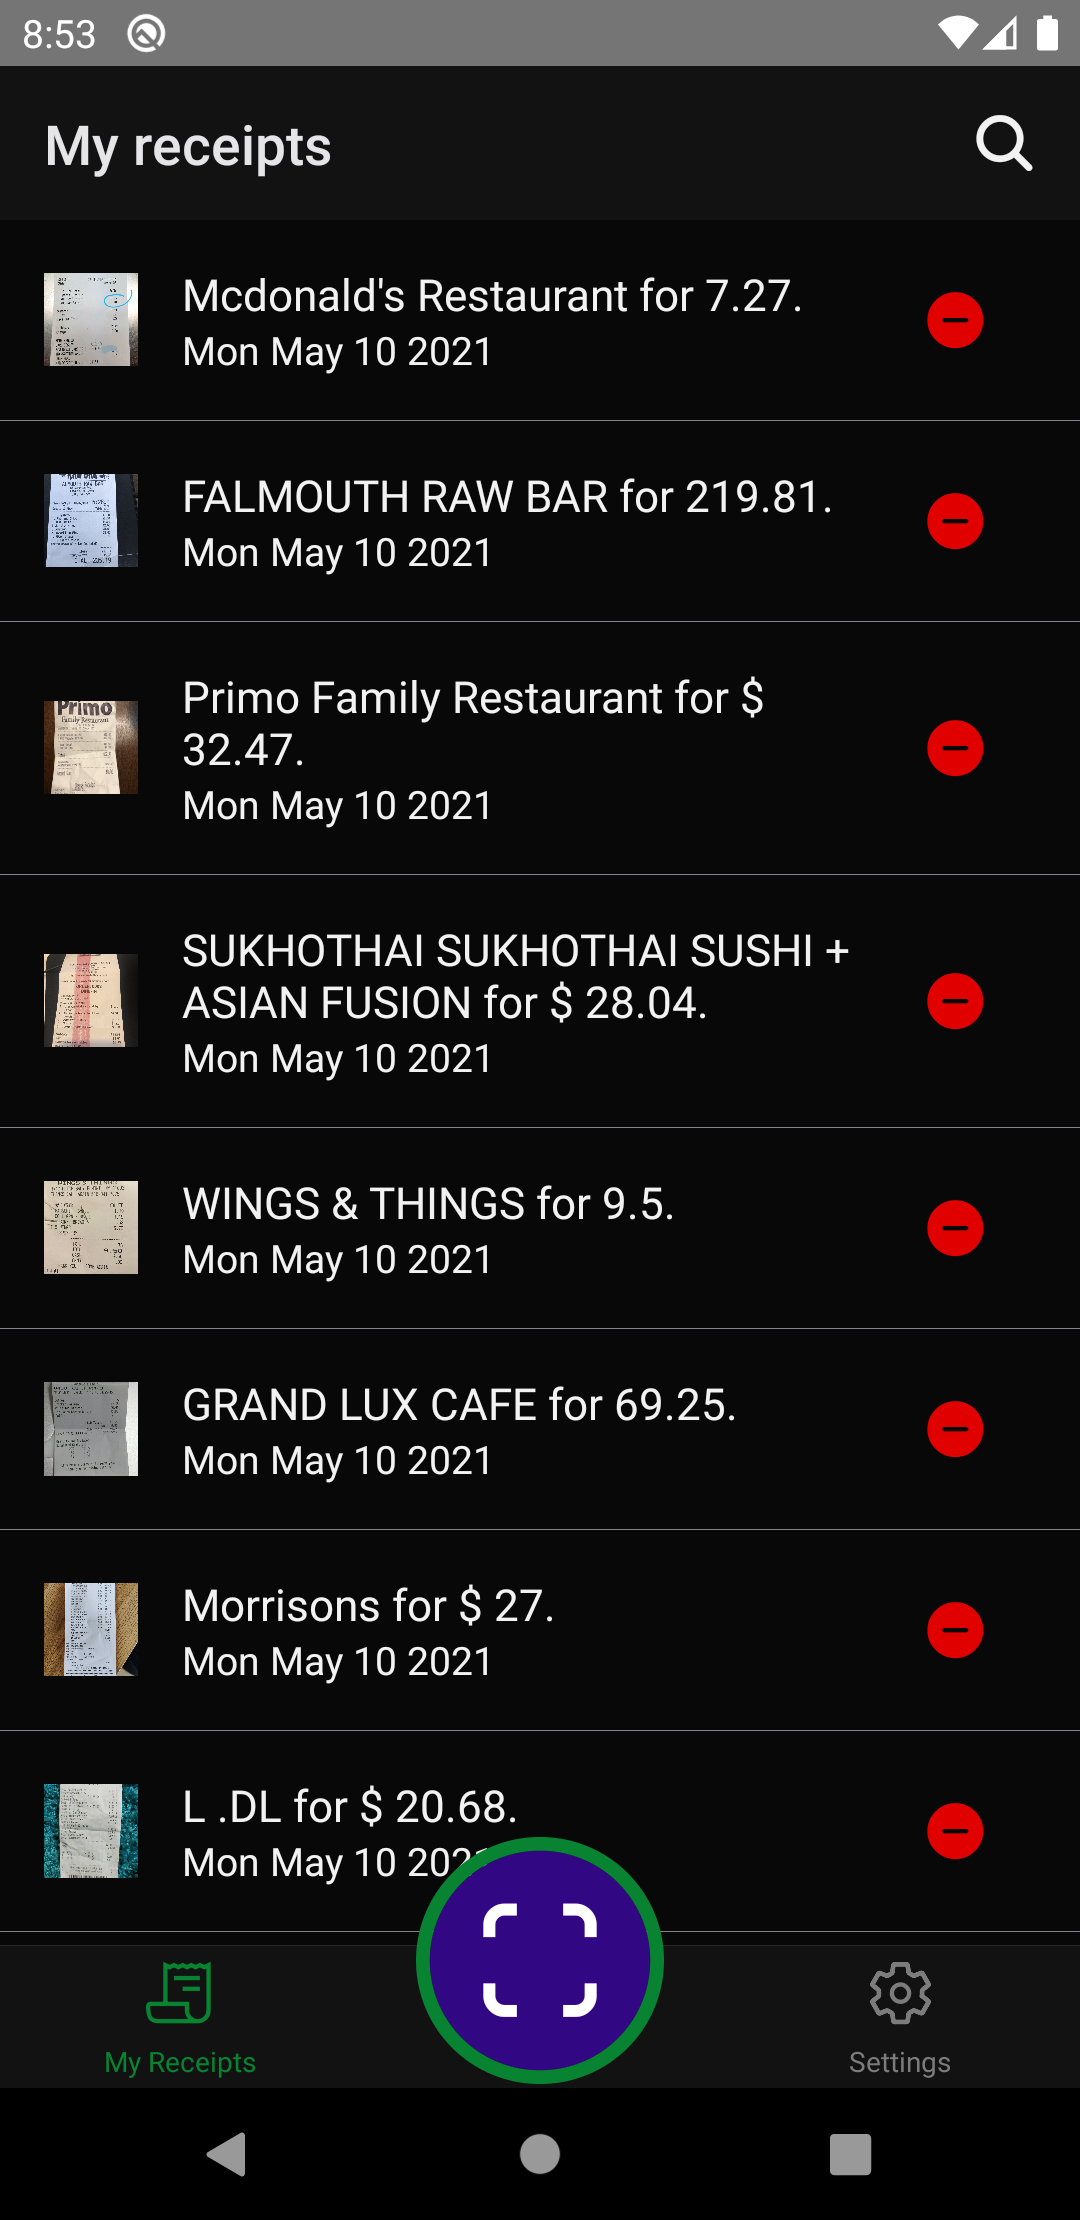
\includegraphics[width=0.95\textwidth]{figures/screens/android/dark/receipts_list}
      \caption{Main application screen showing list of receipts.}
    \end{subfigure}
    \begin{subfigure}[t]{0.5\textwidth}
      \centering
      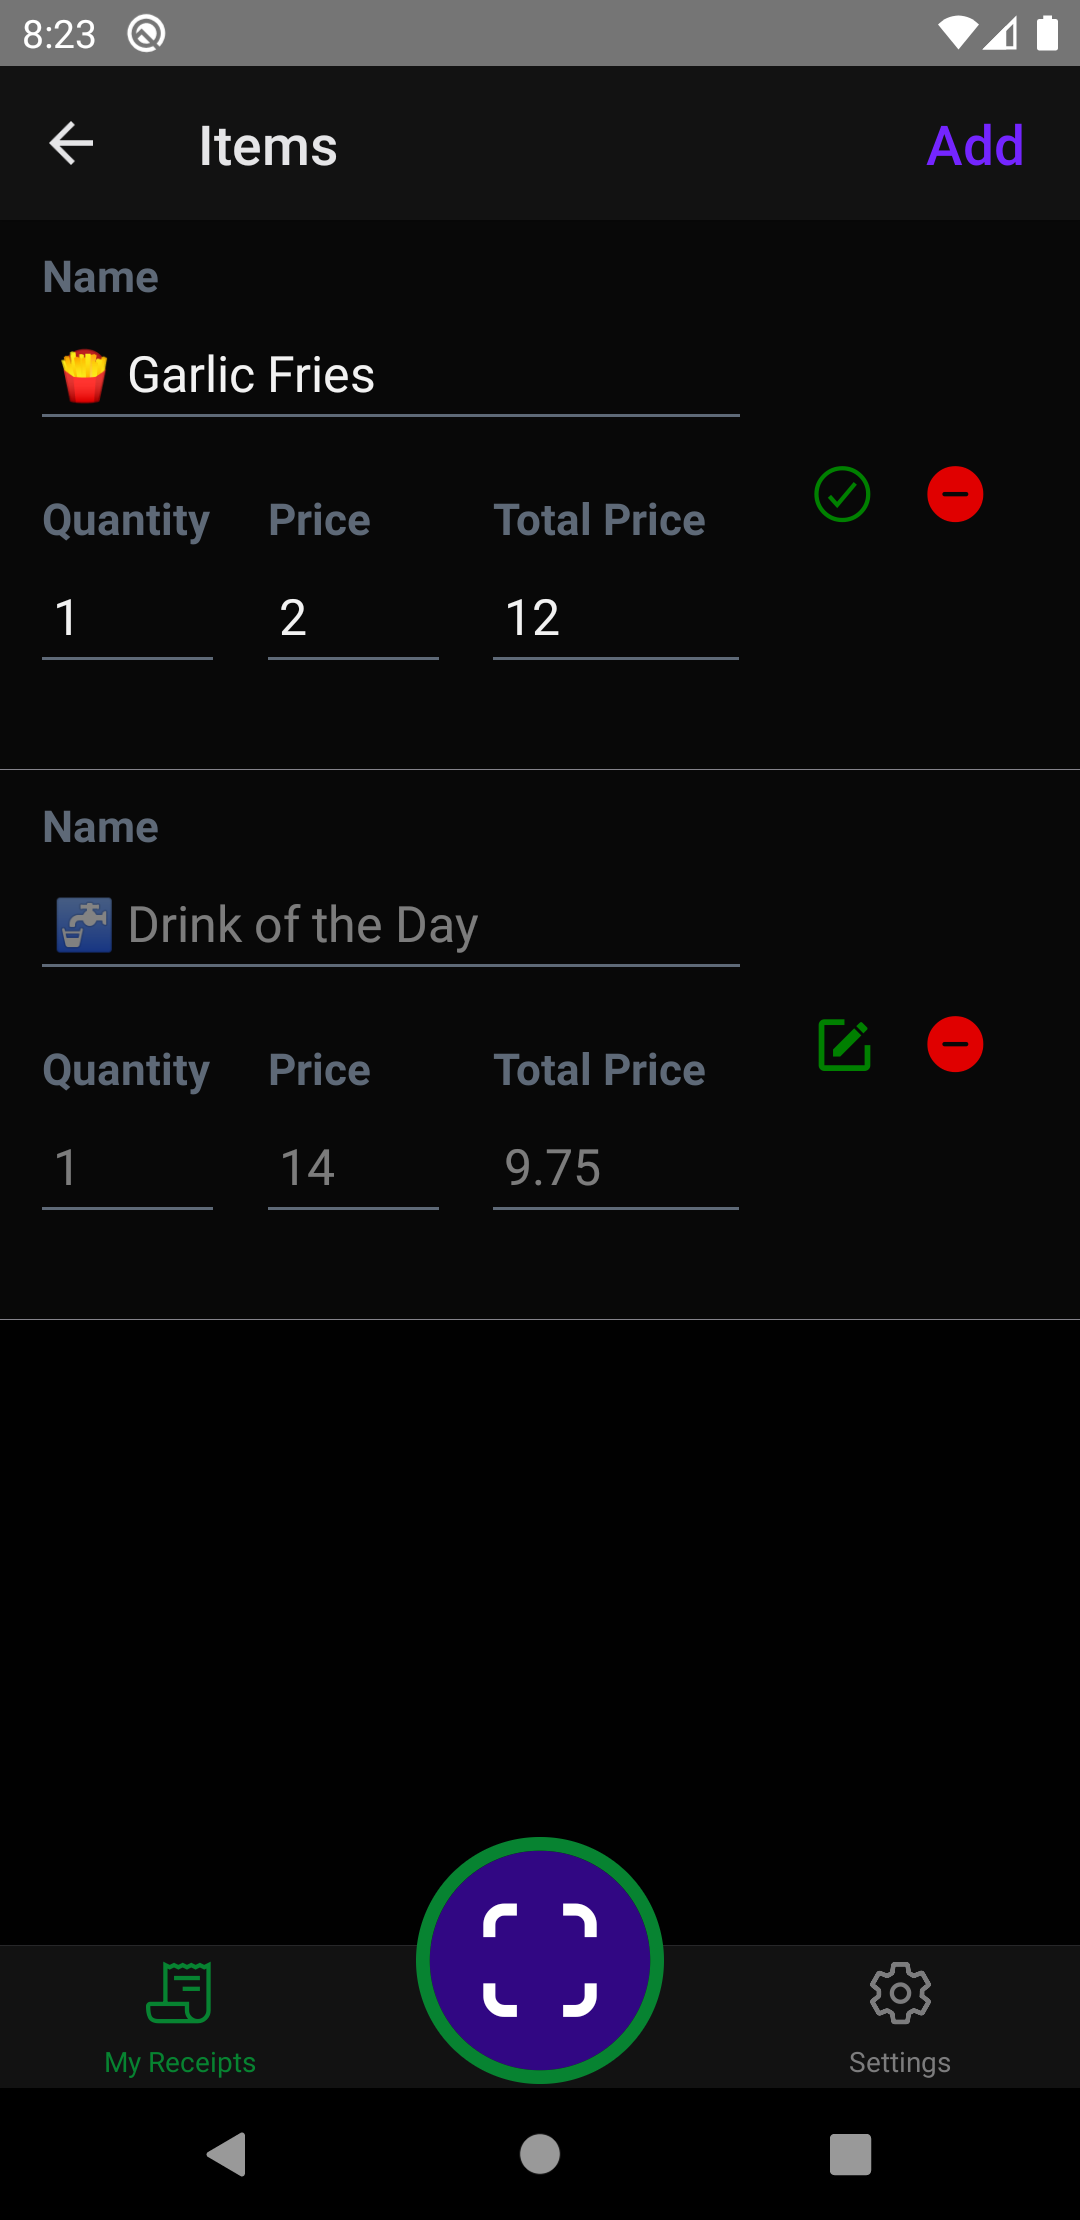
\includegraphics[width=0.95\textwidth]{figures/screens/android/dark/items}
      \caption{A screen with individual receipt items.}
      \label{fig:dark_mode_android}
    \end{subfigure}
    \caption{User interface of Receipts Scanner on Android with enabled dark mode.}
\end{figure}

\begin{figure}
    \centering
    \begin{subfigure}[t]{0.5\textwidth}
      \centering
      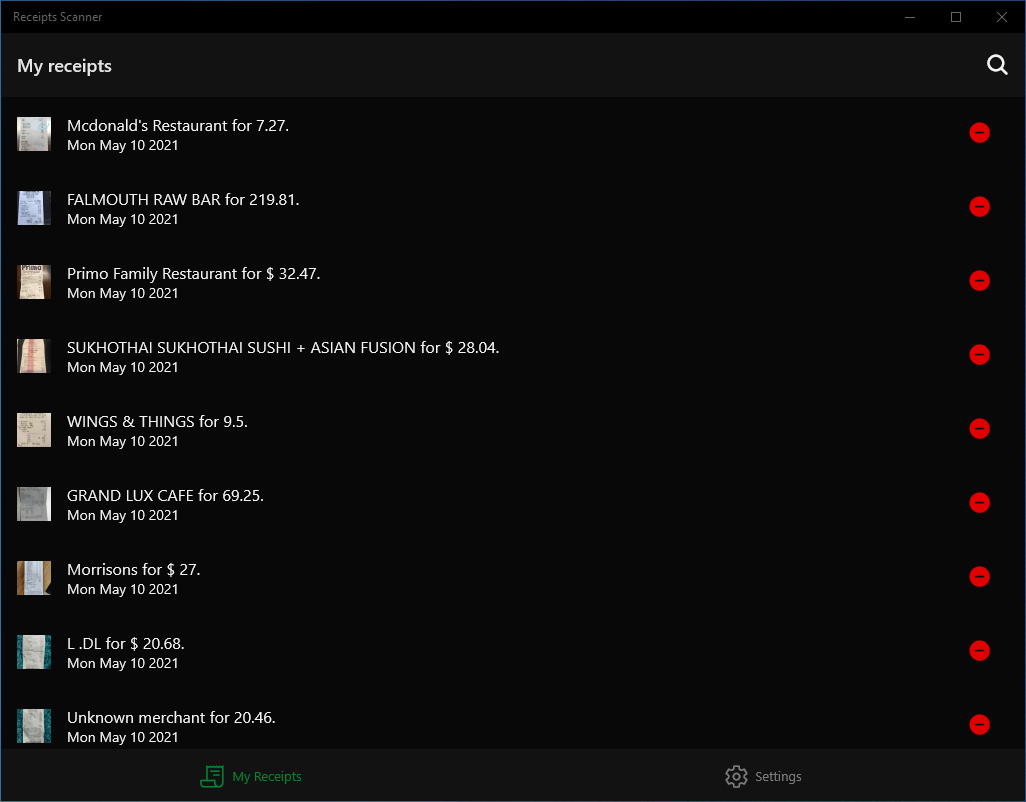
\includegraphics[width=0.95\textwidth]{figures/screens/windows/dark/receipts_list}
      \caption{Main application screen showing list of receipts.}
    \end{subfigure}
    \begin{subfigure}[t]{0.5\textwidth}
      \centering
      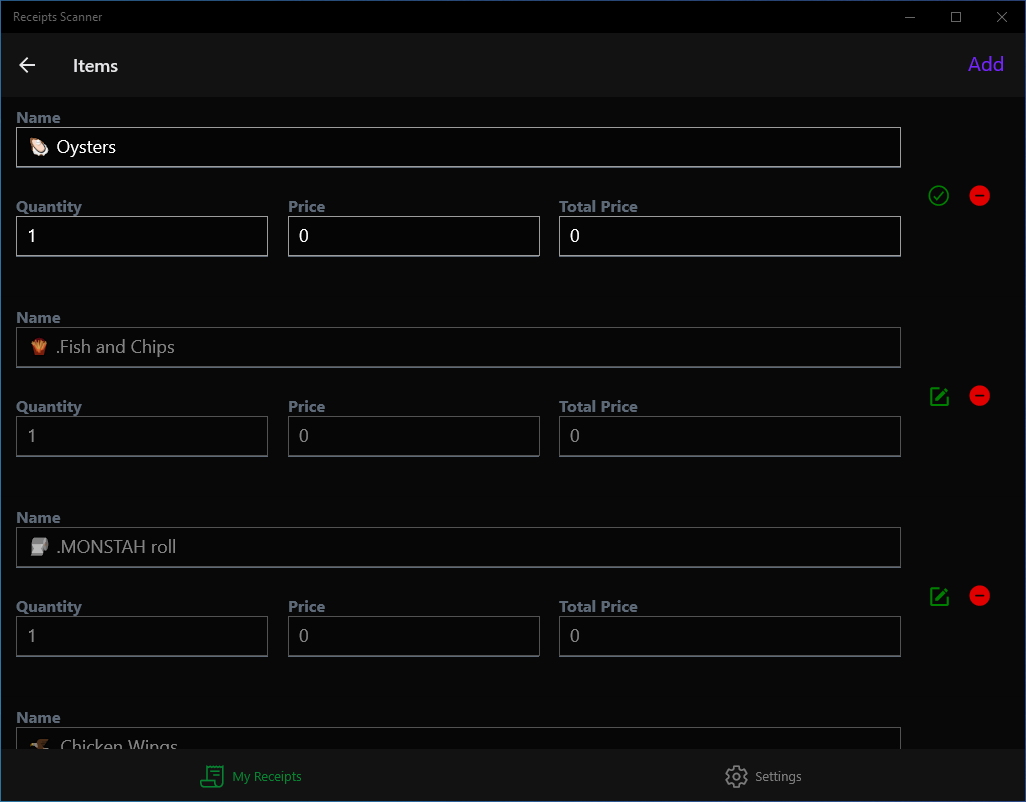
\includegraphics[width=0.95\textwidth]{figures/screens/windows/dark/items}
      \caption{A screen with individual receipt items.}
      \label{fig:dark_mode_windows}
    \end{subfigure}
    \caption{User interface of Receipts Scanner on Windows with enabled dark mode.}
\end{figure}


\chapter{Up to date}
The receipts are always up to date. Any change in the receipt database for a given user is almost instantly reflected on all other devices where that user is logged in. This means that a user can scan a receipt on the mobile and fill the receipt information from the PC. If they decide to delete the receipt, the receipt disappears from the other device as well.
This functionality is possible thanks to Google Firebase.

\chapter{Offline support}
The application works partially offline. If a user is offline and makes any changes to an already existing receipt (edits a receipt, adds a receipt item, deletes a receipt), this change is reflected in the application UI on the device where the changes were made. Once the user connects to the internet, the changes propagate to the database and other devices of the user. The offline changes are persisted even if the application is turned off. This functionality is possible thanks to Google Firebase.

The receipt scanning functionality is not possible in a offline mode. If a user tries to scan a receipt without an internet connection, an alert modal window is shown to them.

Ideally, the image would be stored locally and its thumbnail would be shown among other receipts, but with a status of ‘being processed’. After the device got connected to the internet again, the image would be uploaded and the user could complete the pre-filled form. +

Another approach would be to use a local model, that would extract the receipt data. This way the user could complete the complete journey of adding a receipt at once and the new receipt and its photo would be sent to the APIs later on. 

Microsoft Form Recognizer does not provide an option to export the model, even if it was a custom one. Therefore a different OCR and information extraction approach would be needed. Furthermore, if the offline model was too large, it should be an opt-in feature of Receipts Scanner.


\chapter{Form Recognizer}
Form Recognizer provides a pre-built model that is suitable for recognizing English receipts. It can be accessed through a JavaScript client library \footnote{\url{https://docs.microsoft.com/en-us/javascript/api/overview/azure/ai-form-recognizer-readme?view=azure-node-latest\#recognize-receipts}}. However, this library is built for Node.js runtime, which is different from the React Native runtime. In most cases, React Native uses JavaScriptCore, which is the JavaScript engine that powers Safari \cite{JavaScriptRNEnvironment}.

Receipts Scanner implements a service \texttt{FormRecognizerClient} with the same interface as the one from the official library, but it relies solely on API calls to the Form Recognizer API. The method to extract the information from the receipt is modeled as long-running operation, which means that the initial request returns a URL to which the subsequent requests for the result should be made.

After \texttt{FormRecognizerClient} is created, its \texttt{beginRecognizeContent} method is called with the image that should be processed with the OCR service. The method returns an instance of a \texttt{Poller}. The \texttt{Poller} provides a method \texttt{pollUntilDone} that repeatedly sends requests to the Form Recognizer API until the result is available.

\chapter{Adding a receipt}
The main functionality offered by Receipts Scanner is adding a receipt and storing it in user's collection of receipts.
This process is visualized in Figure \ref{fig:add_receipt_android}.
It starts by user selecting an already existing photo of a receipt from a gallery or taking a new photo with the phone camera. The photo can be cropped to remove the background. It can also be rotated. The rotation does not have any effect on the result of OCR, it affects only how the photo will be shown to the user in their receipts collection.

Next, three sequences of processes happen asynchronously.

The first sequence consists of sending the receipt to Form Recognizer API. The returned data is sent to Python API's \texttt{/category} endpoint where emojis are added to all items that have been recongized on the receipt.

In parallel to this, the image is uploaded to Firebase Storage.

The third sequence starts by sending the image to the \texttt{/process-image} endpoint. The endpoint returns a processed grayscale image that is then uploaded to Firebase Storage.

At the end, the receipt document is added to the user's receipt collection in Firebase Firestore and the edit form is shown. 

The benefit of the asynchonicity of those processes is that the whole process of adding a receipt takes under 8 seconds on average\footnote{Based on measurements of 10 different receipts.}.

\begin{figure}
    \begin{center}
        \includegraphics[width=\textwidth]{figures/diagrams/Add_receipt_Android}
    \end{center}
    \caption{Activity diagram of a user adding a new receipt.}
    \label{fig:add_receipt_android}
\end{figure}



\chapter{Some chapter}
https://www.dtest.cz/nejcastejsi-problemy/musim-mit-pri-reklamaci-originalni-doklad-o-zakoupeni-zbozi/8


„Jako doklad při reklamaci nemusí sloužit jen papírová účtenka, koupě se dá prokázat i originálním obalem, specifičností zboží, které nikdo jiný neprodává, fotkou účtenky a dokonce někdy i svědeckou výpovědí. Nejjednodušší je ale platit za zboží platební kartou. Klient totiž koupi zboží, které reklamuje, může doložit také bankovním výpisem, kde je uveden název obchodníka, datum nákupu a částka, kterou zaplatil,“ uvedla Iva Haiderová z právního oddělení Air Bank.
Zdroj: \url{https://www.lidovky.cz/byznys/firmy-a-trhy/uctenku-nepotrebujete-vetsina-cechu-nezna-sva-prava-pri-reklamaci-ukazal-pruzkum.A181212_113402_firmy-trhy_pkk}
https://www.coi.cz/faq/5-potrebuji-k-reklamaci-kupni-doklad/

Reklamovat můžete i bez originální účtenky! Prodejci obvykle požadují vrátit zboží v původním nepoškozeném obalu, ale trvat na tom nesmí. Podmínkou reklamace je dokázat, že jste zboží u prodejce koupili, např. výpisem z účtu při platbě kartou nebo bankovním převodem. Koupi lze prokázat i originálním obalem či specifičností zboží, které nikdo jiný neprodává. V některých případech může pomoct i výpověď svědka.
https://smoneybox.com/cs/blog/reklamace-jak-spravne-reklamovat-vadne-zbozi

Musím při reklamaci mít prodejní doklad („paragon“)?
De iure ne, de facto to může být nezbytné. Žádný zákon vám tuto povinnost neukládá, musíte ale prodejci dokázat, že jste věc koupil u něj, resp. kdy. Toto můžete doložit i pomocí svědků, prodejce to ale nemusí uznat a pak nezbývá, než se soudit. Skutečnost a datum prodeje můžete doložit např. také záručním listem, pokud vám byl vystaven. I v tomto případě však ještě zůstává problém doložení kupní ceny pro případ odstoupení od smlouvy. Prodejce je ale u spotřebního zboží (nikoliv u služeb) dle §11/2 Zák. o cenách povinnen uchovávat cenovou historii 3 roky a mimo to má možnost zjistit cenu z účetních dokladů, jejichž uchování mu předepisuje zákon o účetnictví. Dobrou vůli k prokázání ceny však nelze předpokládat.
https://businesscenter.podnikatel.cz/pravo-predpisy/ochrana-spotrebitele/otazky-a-odpovedi-spotrebitelskeho-prava/

\chapter{Creating a new application}
The official way of creating a new React Native application is to use React Native CLI\footnote{Command Line Interface}. The application produced by the CLI contains only one component. It does not use any additional libraries apart from the linter\footnote{A static analysis tool that highlights errors and enforces good programming practices.} and a testing framework.

The process of developing applications with React Native is often repetitive and the same setup needs to be made for every application. To reduce the time it would take to install all required libraries and to enforce the best practises, application boilerplates have been created.

\section{Ignite}
The most used boilerplate for React Native is Ignite\footnote{See \url{https://github.com/infinitered/ignite}.}.
Ignite is a CLI and an application boilerplate at the same time. It is opinionated, meaning that it enforces certain project structure and libraries. Navigation, application state management, Storybook component library, Detox end-to-end tests and Reactotron (for inspecting the application) are already set up. The CLI can be used for generating new components and screens.

\section{Expo}
Expo\footnote{See \url{https://docs.expo.io/}.} is a framework built on top of React Native. An application created with Expo CLI can be run on iOS, Android and Web. It provides many external tools that help with the development process. 
Many libraries for React Native have been created by Expo. Those libraries can be often used also in applications that do not run on Expo.

It is not possible to add a React Native for Windows to the Expo project. For this reason, Receipts Scanner was set up with the React Native CLI instead.

It is very likely that Expo will support React Native for Windows in the future\footnote{Feature request to support React Native for Windows in Expo: \url{https://expo.canny.io/feature-requests/p/support-for-react-native-windows-apps}.}.

In the meantime, the Expo built for Web could be run on Windows using Electron.

\chapter{Development}
\section{Component library}
When developing a React application, it is a good practise to have a set of basic components from which more complex ones are built up. The set of those basic components is called a component library or a design system. An efficient way of building the component library is by using a tool


that allows development of each component in isolation.

Storybook\footnote{See \url{https://storybook.js.org/}.} is a widely used tool for developing UI components in isolation. It is based on plugins. Thanks to its open-source nature, there are many plugins created by the community, which extend the core functionality of Storybook.

Storybook is based on the concept of stories. A story is a permutation of the component with given properties. Each component can have multiple stories. A \texttt{Button} component could have one story displaying the Button in its \textit{enabled} state and a second one for the \textit{disabled} state.

Storybook stories serve as a gallery of available components and a documentation of their properties. They can be used for snapshot and visual tests, which are described in Sections \ref{sect:snapshot_testing} and \ref{sect:visual_testing} respectively.

Storybook exists both in React and React Native version. 
Whereas Storybook for React runs in a web browser, Storybook for React Native needs to run on a mobile device, because React Native uses native components that cannot be displayed in the browser. 

Running Storybook on a mobile device is achieved by rendering the Storybook component instead of the root component that would normally be rendered. In order not to have to replace the component manually in code every time, Receipts Scanner takes advantage of Reactotron\footnote{See \url{https://github.com/infinitered/reactotron}}. Reactotron is a desktop application that provides a suite of tools for easier development in React Native. It is integrated inside the project, so it is possible to switch between displaying Storybook and the actual application from the Reactotron UI. 

Figure \ref{fig:storybook_rn} shows how the component library and the interface of Storybook for React Native look like.

\begin{figure}
    \centering
    \begin{subfigure}[t]{0.5\textwidth}
      \centering
      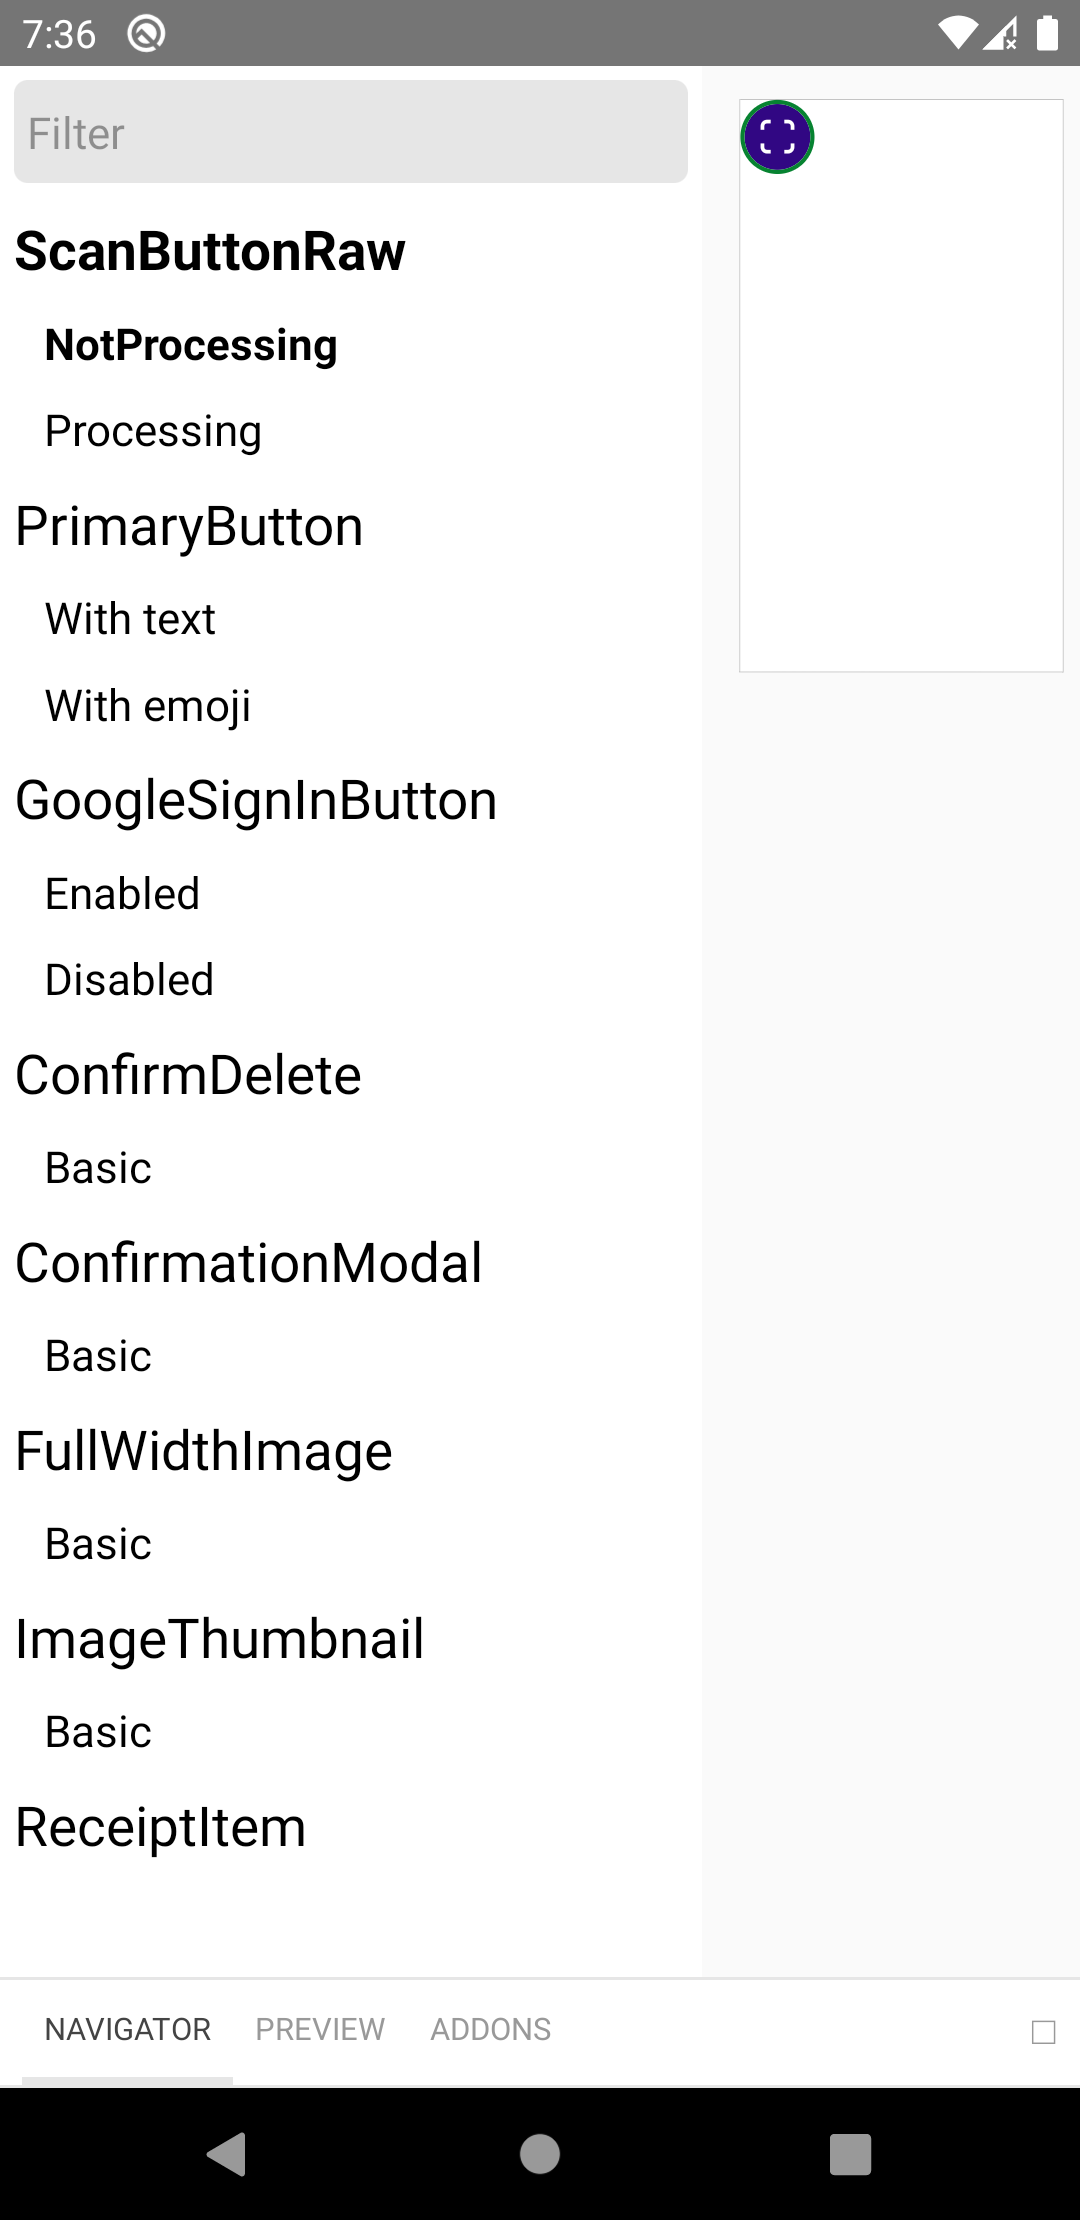
\includegraphics[width=0.95\textwidth]{figures/other/storybook_rn_menu}
      \caption{Menu of components.}
      \label{fig:storybook_rn_menu}
    \end{subfigure}%
    \begin{subfigure}[t]{0.5\textwidth}
      \centering
      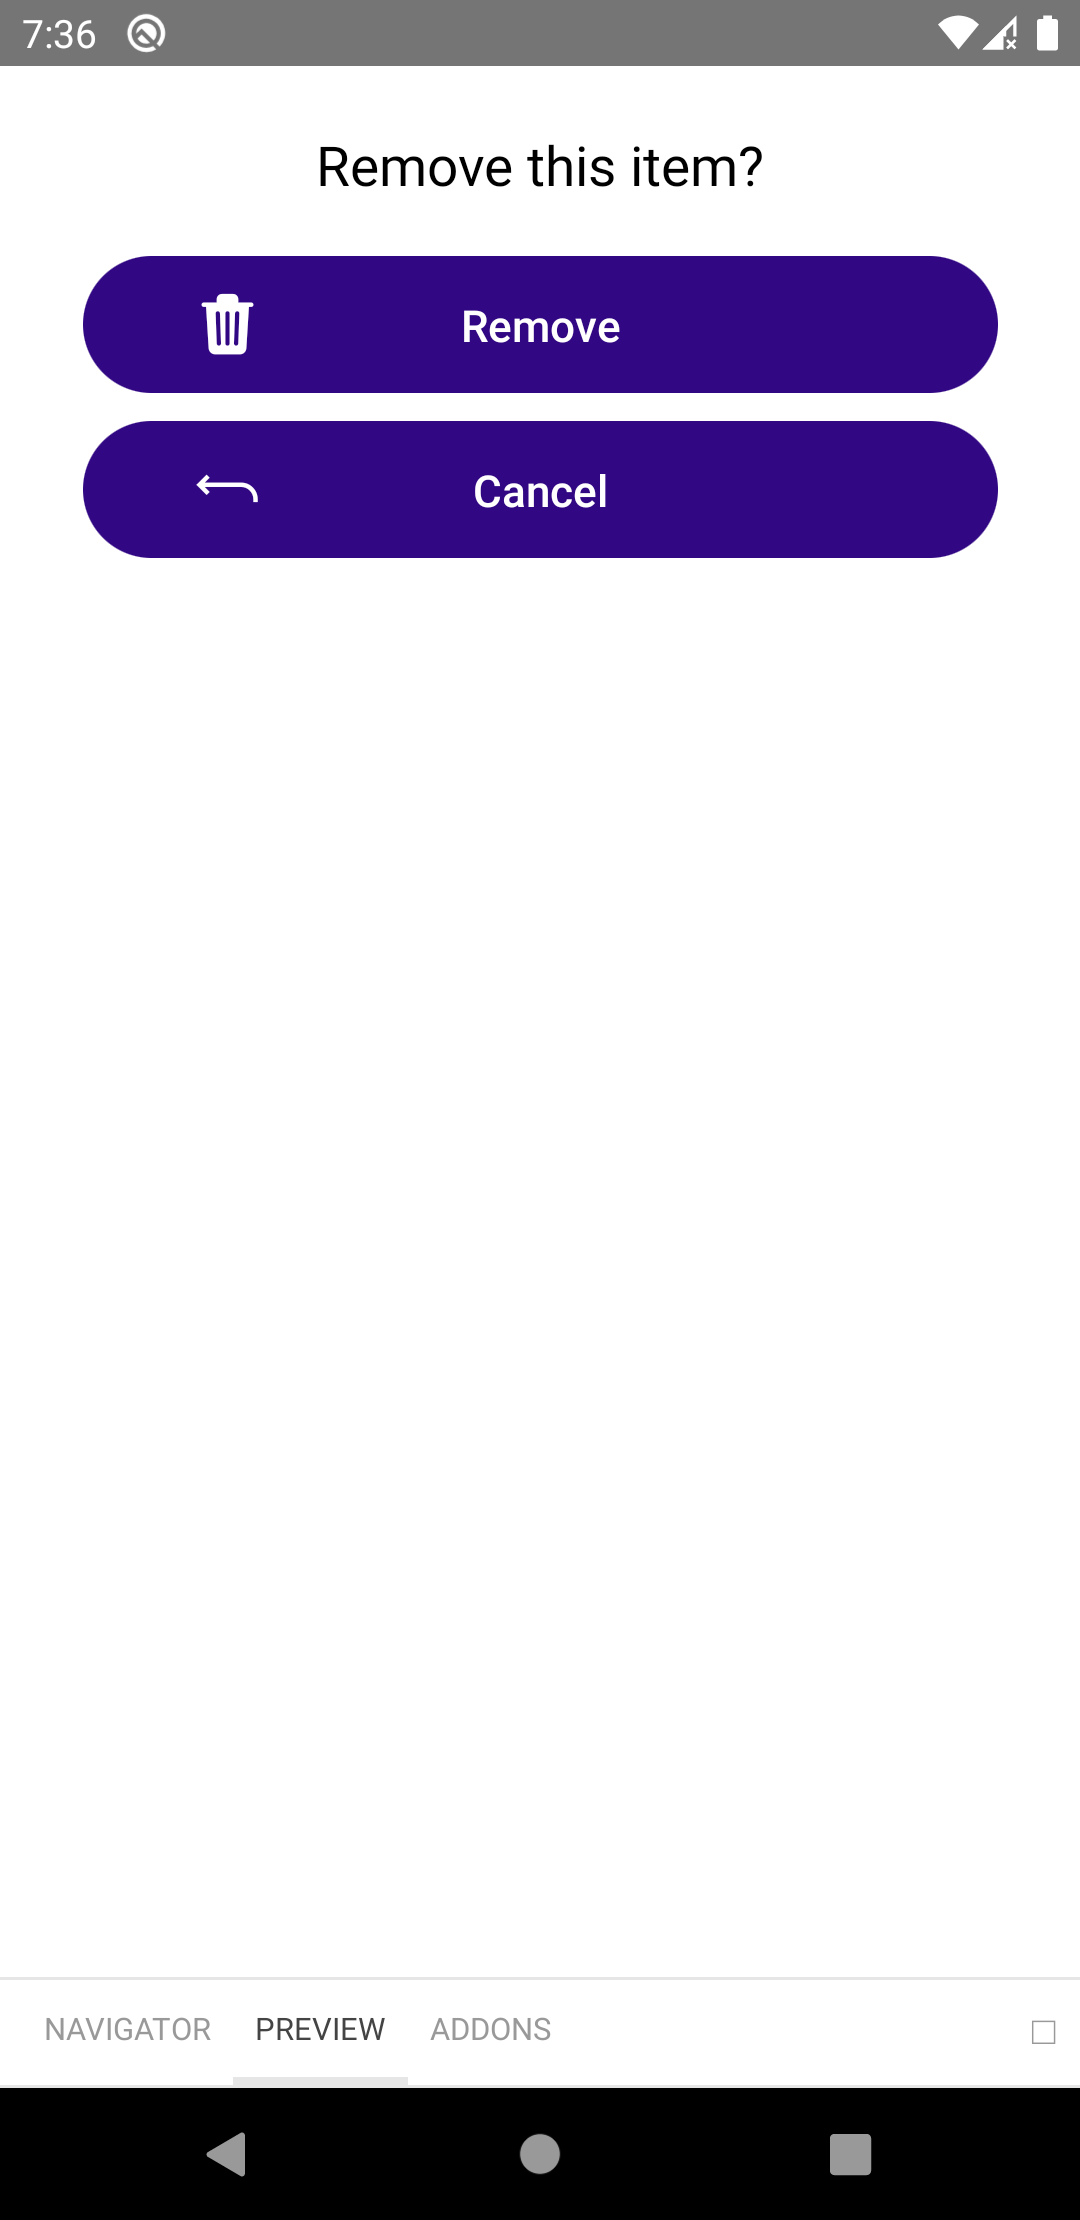
\includegraphics[width=0.95\textwidth]{figures/other/storybook_rn_confirm_delete_component}
      \caption{Detail of \textit{Confirmation Dialog} component.}
      \label{fig:storybook_rn_confirm_delete_component}
    \end{subfigure}
    \caption{Login screen.}
\end{figure}
\label{fig:storybook_rn}


It is possible to install a Storybook server that enables navigation between stories directly in the browser. However, the stories are still displayed only on the mobile device. In order to show the stories in the browser a react-native-web\footnote{See \url{https://necolas.github.io/react-native-web/}.} library can be used. There are two options:
\begin{enumerate}
    \item Alias react-native imports to react-native-web in the bundling\footnote{Bundling is the process of transpiling all source files and assets of the application, usually into one large JavaScript file that can be run across different browsers.} process of the whole app. This makes the whole application able to run in the browser. The Storybook functionality is therefore a side-effect.
    
    The Expo applications can run in the browser by default, no extra configuration is necessary to have Storybook for React Native running in the browser.
    
    \item Install Storybook for React. Alias react-native to react-native-web in the bundling process of Storybook. This approach is used in Receipts Scanner. Figure \ref{fig:storybook_web} shows how the component library and the interface look like.
    
    An advantage of this approach is that even though Storybook for React Native is in version 5, the Storybook for React can use the latest version 6. The version 6 is able to find all stories in the projects automatically without having to list each story explicitly. It also uses more concise and more intuitive syntax of writing stories.
    
    Another advantage is that the Storybook created by this approach can be used with libraries for web development, such as Chromatic for visual testing. It can be built into static files and served as a application independent of the React Native application.
    
    The main disadvantage is that there are two separate Storybooks in the project. A small amount of extra code needs to be written for each story to make it visible in both Storybooks. 
    
\end{enumerate}

\begin{figure}
    \begin{center}
        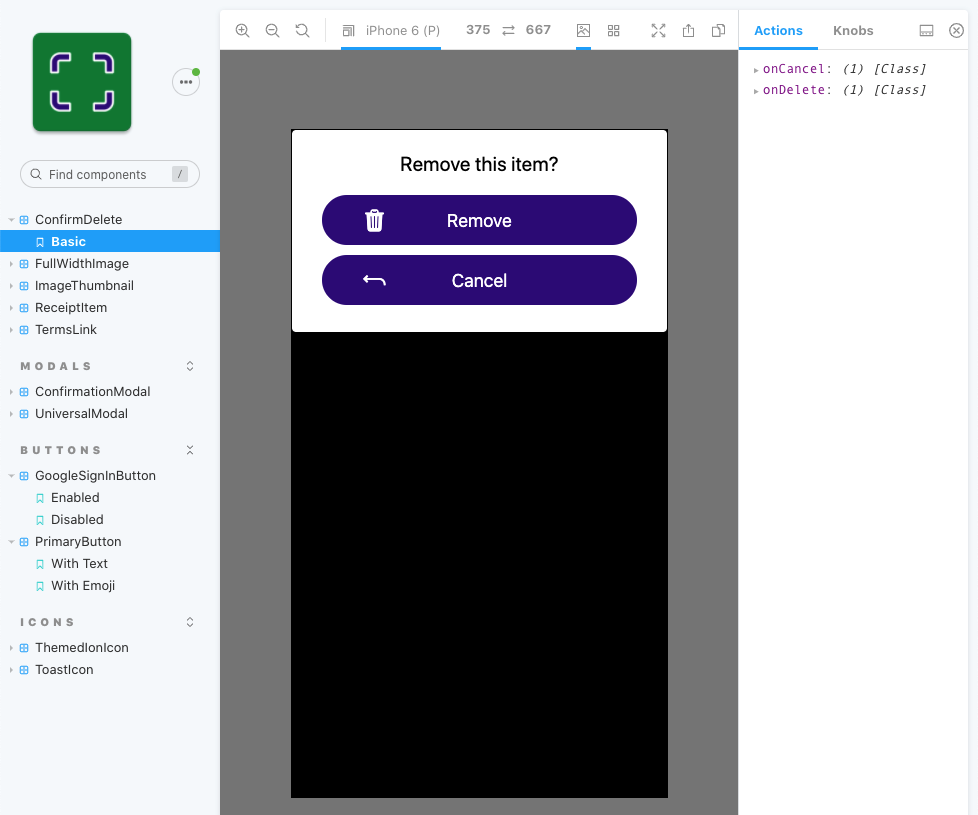
\includegraphics[width=\textwidth]{figures/other/storybook_web}
    \end{center}
    \caption{Storybook for React in the browser.}
    \label{fig:storybook_web}
\end{figure}

\chapter{Testing}
The Receipts Scanner uses five kinds of tests: unit tests, component tests, snapshot tests, visual regression tests and end-to-end tests.
The former three use a JavaScript testing framework Jest\footnote{\url{https://jestjs.io/}}.

\section{Unit tests}
Unit tests test individual functions. Their main goal is to assure that the utility functions such as RGB to HEX color conversion or receipt filtering works.

\section{Component tests}
Component tests test individual React components. An example could be a test for a \textit{Receipts List} component. Let us assume that the component calls an API and displays the returned receipts. The test would mock the API call, return fixed list of receipts and assert, that those receipts are visible.

In React Native, there is an option to choose between two libraries, react-test-renderer and React Native Testing Library. 

react-test-renderer renders components to pure JavaScript objects without depending on the DOM\footnote{Document Object Model} or a native mobile environment. It provides methods for locating elements for example by component type (e.g. Text) or properties (e.g. finding a button with \texttt{title} value equal to \textit{Submit}.

It is possible to get the rendered component as a JSON and use it for snapshot testing, which is described in the next section \ref{sect:snapshot_testing}.

The issue of testing with react-test-renderer is that the tests rely on implementation details of the components.

React Native Testing Library solves this problem by providing utility functions on top of react-test-renderer for locating elements for example by the visible text or accessibility label, so the tests resemble how users interact with the application. It is inspired by React Testing Library, which is a widely used testing library for React. \cite{TODO}
%https://reactjs.org/docs/test-renderer.html
%https://trac.webkit.org/wiki/JavaScriptCore
%https://reactjs.org/docs/test-renderer.html
%https://callstack.github.io/react-native-testing-library/docs/getting-started
%https://callstack.github.io/react-native-testing-library/docs/how-should-i-query


\section{Snapshot testing}
\label{sect:snapshot_testing}
Snapshot tests verify that the rendered markup of the components stays the same. When the snapshot tests are run for the first time, the rendered markup is saved in a file.
During subsequent runs, the newly rendered markup is compared to the saved one. The tests fail when there is a differences between the two. Those differences are usually highlighted for the developer to asses, whether or not this change was intentional. If it was, the saved snapshots are updated. Otherwise the unintentional changes are fixed.

It is possible to create snapshot tests with Jest and react-test-renderer by rendering the component to JSON and comparing it to the previously rendered version \footnote{TODO \url{https://jestjs.io/docs/snapshot-testing}}.

This process can be automated with Storybook.
By using a Storybook addon StoryShots\footnote{\url{https://www.npmjs.com/package/@storybook/addon-storyshots}}, all stories in the project are turned into snapshot tests. 

This is a very efficient and inexpensive way of testing, because the stories most of the time already exist.

Snapshot testing catches only changes in markup. This does not include any style changes. If the CSS or an image change, the snapshot tests will still pass. 

On the other hand, changing markup does not necessarily mean that the result is different. It is very often the case, that even though the markup has changed, the page looks the same as before and the tests report false positives. For these reasons, snapshot tests can be quite brittle.

\section{Visual testing}
\label{sect:visual_testing}
Visual testing addresses the issues of snapshot testing mentioned earlier. It is not important if the markup changed. The important thing is whether the component looks as desired. Visual tests, also called visual regression tests, provide an assurance that once the expected look of a component was achieved, it will stay unchanged.

Visual testing is a process of comparing screenshots of newly rendered components with the old screenshots, also called reference images.
When visual tests are first run, a set of screenshots is made. During subsequent runs, those screenshots are compared to the stored ones. Possible differences are highlighted. There are various tools that can highlight the differences between images. Those tools can be independent of those that are used to take the screenshots.

A widely used tool for visual testing in React community is Chromatic. It creates screenshots of the Storybook stories. It is not possible to use Chromatic with Storybook for React Native. Since Receipts Scanner has also a Storybook for React component library created by utilizing react-native-web, the Chromatic is used for testing components there.

Chromatic runs in the continuous integration pipeline (CI pipeline)\footnote{A series of steps that are executed when changes are pushed to the remote project repository.}. The changes need to be reviewed on the Chromatic website created for given CI run. Chromatic also publishes the Storybook as a website.

Figure \ref{fig:chromatic_diff} shows how the review process of a visual change in Chromatic UI looks. Both the visual change and the change in the markup are visible.

\begin{figure}
    \begin{center}
        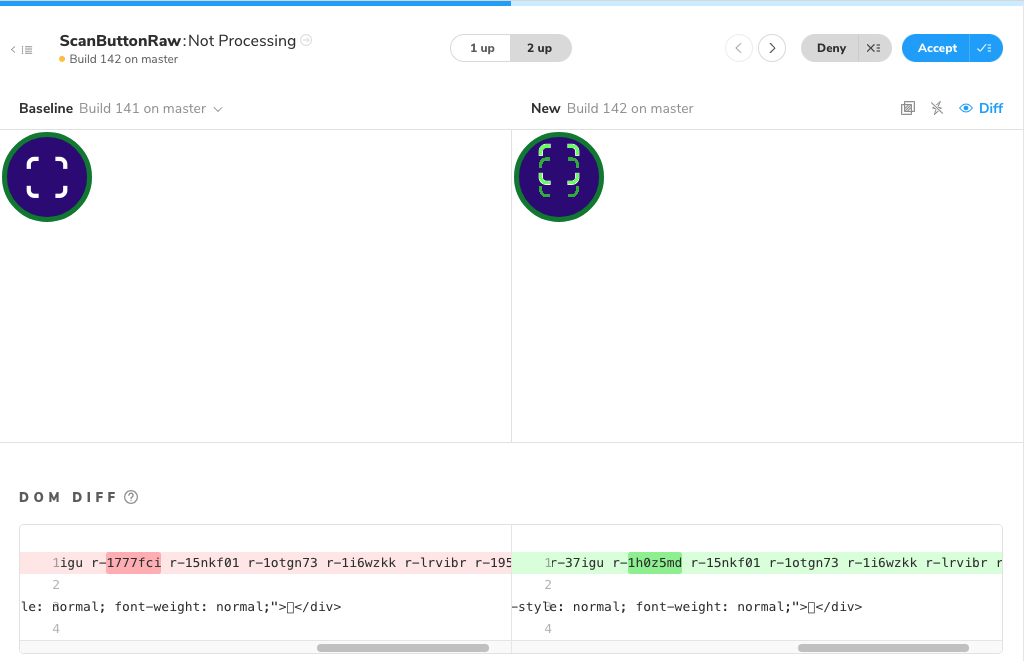
\includegraphics[width=\textwidth]{figures/other/chromatic_diff}
    \end{center}
    \caption{Chromatic screen for reviewing visual change of the \texttt{ScanButtonRaw} component. The Scan icon moved up.}
    \label{fig:chromatic_diff}
\end{figure}

An alternative to Chromatic is a tool called Loki, which also integrates with Storybook. It is able to take screenshots in a Chrome browser, on iOS simulator or on Android emulator, which means it can be used both with Storybook for React and Storybook for React Native.

Loki creates difference images which highlight the visual change. A visual change of scan button component is shown in Figure \ref{fig:loki_diff}.

\begin{figure}
    \begin{center}
        
\includegraphics[width=0.3\textwidth]{figures/other/loki_diff}
    \end{center}
    \caption{Image generated by Loki indicating a visual change to the \texttt{ScanButtonRaw} component. The Scan icon moved up.}
    \label{fig:loki_diff}
\end{figure}

I would not recommend using Loki for Storybook for React Native. The tests are unstable and the screenshots differ even though the component itself has not changed. This is caused by the component not being fully loaded when the screenshot is made. Loki uses running Storybook server for controlling which story is shown, which sometimes does not work, resulting in flashing between different stories.
Loki performs better with Storybook for React, but it cannot take screenshots of modal components.

A third approach of visual testing I tried was a combination of Storycap and RegSuit. Similar to Chromatic, this works also only with Storybook for React.

First, Storycap takes screenshots of the stories. Reg Suit then downloads the previous screenshots from Google Cloud Storage, compares them with the new ones and stores the differences. 

Storycap and Reg Suit should run in the CI pipeline. From my experience, Reg Suit had problems determining the hash of the previous commit. This hash is used to pick correct images from the Google Cloud Storage bucket for comparison. For this reason, all stories were being reported as new and no comparison happened.

Naturally, it is not good to use all three solutions for visual testing together. I would suggest using only Chromatic, because it has the fastest setup, it is the most reliable one and provides the best user interface for reviewing the changes.

TODO linky, zdroje

Similarly to snapshot tests, the visual tests are created automatically from stories. The visual testing is therefore very convenient.

\section{End-to-end testing}
End-to-end tests are used to test a user interaction with the application from the beginning to the end. 

An example of an end-to-end test would be testing of the sign in functionality, i.e. after the required fields of the sign in form are filled in and the \textit{Sign in} button is pressed, a screen for the authenticated users is shown.

Multiple end-to-end testing frameworks for React Native exist.
Receipts Scanner is setup for testing with Detox. However, there are only a few end-to-end tests. Despite Detox being a popular choice for React Native testing, mostly for its speed compared to other options, the tests often fail nondeterministically.

A more recent project, Cavy\footnote{\url{https://cavy.app/}}, takes a different approach from Detox. It does not use any native code, all functionality is achieved with pure JavaScript. The setup is therefore easier but the functionality is limited. 

Whereas Detox is able to locate elements by text or label, Cavy needs that each component that is being tested is wrapped with a special function. This creates a noise in the code.

The oldest testing framework of the ones mentioned is Appium\footnote{\url{http://appium.io/}}. Similar to Selenium WebDriver\footnote{Selenium is a software for automated testing of web applications.}, it uses WebDriver protocol\footnote{WebDriver protocol is used to control the browser.}. It could be used for testing both Android and Windows version of the Receipts Scanner. 

\subsection{Mocking native modules}
In unit, component and snapshot tests, the native modules need to be mocked. The testing framework Jest can run only JavaScript code.

Visual tests require Storybook to be running. If the Storybook is running on Android device, no mocking is necessary. If Storybook for React is used for visual testing, the modules that do not have Web support need to be mocked as well.

The components can be divided into two categories -- pure and connected. Pure components are components that display data based on their properties. Connected components connect to the database, make API calls and depend on native modules. They pass the data to pure components. In general, stories should be written for pure components, therefore no mocking of native modules should be needed.

\subsection{Continuous integration}
Continuous integration is a practise of frequently merging code changes into a central repository. The changes are validated by creating a build and running automated tests. \cite{fowler2006}

Receipts scanner takes advantage of GitHub Actions. Every time new code is pushed to the main branch of the GitHub repository, three workflows are run. A workflow consists of multiple jobs that run in parallel. Each job consists of multiple sequential steps.

During the first workflow,
\begin{itemize}
    \item the code is checked for any linting or type errors,
    \item a suite of unit and snapshot tests runs,
    \item Storybook is deployed and visual tests run,
    \item a release version of Android application is built,
    \item a release version of Windows application is built.
\end{itemize}

The second workflow runs end-to-end tests on an emulated Android device.

The third workflow runs tests of the Python API. The Python API deployment logic is not contained in the workflows. Instead, a repository hook is setup in the Google Console\footnote{A user interface to manage services provided by Google.} to deploy the latest version of the Python API.

\chapter{Features}
This chapter provides an overview of the functionality available in the Receipts Scanner. Unless stated differently, the same feature is available on both platforms, i.e. Android and Windows.

\begin{enumerate}
    \item Authentication
        \begin{enumerate}
            \item Sign in / sign up with email
            \item Sign in / sign up with Google -- only Android
            \item Email format validation
            \item Password length validation
            \item Preview of password in plain text on toggle 
        \end{enumerate}
    \item Adding of receipt -- only Android
        \begin{enumerate}
            \item Selecting the receipt from gallery
            \item Taking a picture of the receipt directly from application
            \item Receipt image cropping and rotation
            \item Automatic data extraction from the photo of a receipt and form pre-filling
            \item Automatic adding of emojis to each receipt item
        \end{enumerate}
    \item Receipt preview
        \begin{enumerate}
            \item Preview of the original image
            \item Preview of a processed image for better readability
            \item Purchase date, merchant name, merchant address, merchant phone number, total price, subtotal, tax, tip and currency.
            \item List of receipt items with emoji, name, quantity, price and total price.
        \end{enumerate}
    \item Receipt editing
        \begin{enumerate}
            \item Editing of purchase date, merchant name, merchant address, merchant phone number, total price, subtotal, tax, tip and currency.
            \item Form fields validation
            \item Ability to move between form fields using only keyboard
            % TODO check windows
            \item Receipt item adding
            \item Receipt item editing
            \item Receipt item deletion
        \end{enumerate}
    \item Searching through receipts by merchant name, merchant address and individual receipt items
    \item Receipt deletion
    \item Dark mode that reflects system settings
    \item Partial offline support
    \item Internet connectivity notification -- mocked on Windows
    \item Export of receipts data and images
    \item Notification toast messages
\end{enumerate}

\chapter{Native Modules}
Native modules provide an access to the native platform API that is not available by default in JavaScript \cite{RNNativeModulesIntro}, for example an API to select a picture on the device. Another reasons for using native modules are taking advantage of existing native libraries or running multi-threaded code.

Native modules for Android are written in Java or Kotlin.
For Windows, they can be writter in C++ or C\#, but C++ is the preferred language, mostly due to its performance.

Native modules can be written directly in the application or added as an external package. React Native Directory\footnote{See \url{https://reactnative.directory/}.} provides a list of available native modules. They can be filtered by the supported platform, because very often, the native module is not available on all platforms which are supported by React Native. This is the largest drawback of using React Native in my opinion. 

In case a native module is not available on a given platform, there are four available options:
\begin{enumerate}
    \item \textbf{Omitting the module.} If the functionality provided by the native module is not critical, it might be omitted on a given platform. This is possible by having a different code for each platform. This concept is described in Chapter \ref{chap:platform_specific_code}.
    
    In Receipts scanner, this approach has been taken with Google Sign In, which is not available on Windows.
    
    \item \textbf{Mocking the module.}
    This approach has been applied in Receipts Scanner on NetInfo module, which provides information about the internet connection. Currently, it is not possible to use it on Windows\footnote{GitHub issue: \url{https://github.com/react-native-netinfo/react-native-netinfo/issues/306}.}. Therefore it has been temporarily mocked to always return information about the device being online.
    
    \item \textbf{Replacing the module.} In case a different module that provides q similar functionality is available, it can be used instead. If such module does not exist, it can be implemented.
    
    Receipts Scanner implements its own \footnote{FilePicker} module to provide functionality of picking an image from the file system on Windows.
    
    \item \textbf{Adding the missing platform to the module.}
    Most of the modules are open-source projects to which anyone can contribute. React Native is a relatively new ecosystem and relies on community contributions. In general, anyone can add a new platform to an existing library.
\end{enumerate}

\chapter{Choice of platforms}
\label{chap:choice_of_platforms}
According to Pew Research Center \cite{PewResearchCenter2021}, 85\% of adults in US own a smartphone (as of 2021). There is no dispute about smartphone being a ubiquitous device in people's lives. 
Most smartphones have a decent camera that allows taking photos of receipts in a sufficient quality. Therefore most of the focus has been on developing a mobile app.
The next question that needs to be answered is whether to target Android, iOS or both. According to IDC's market research \cite{Idc2021}, in 2020, 84.1\% of smartphones were equipped with Android and 15.9\% with iOS. Development of iOS applications requires a Mac\footnote{Mac, also known as Macintosh, is a family of personal computers sold by Apple. Current models include MacBook Pro and iMac.} and Xcode\footnote{Xcode is a software by Apple for developing applications for Apple products. See \url{https://developer.apple.com/xcode/}.}. There exist some workarounds around this limitation, but most of them rely on using a Mac in the cloud. At the beginning of writing of the thesis I did not have an access to Mac. In order to be able to target more devices and also given the mentioned limitation, I chose to develop and Android application.

Although smartphones are convenient for taking the photo of the receipt right after the purchase, some users might prefer a desktop application to view and search the receipts.
According to Statcounter \cite{Statcounter2021}, Windows makes for the 75.55\% of desktop operating systems, OS X comes second with 16.5\%\footnote{Data have been collected based on website views.}.
For the same reasons (ability to cover more devices and having Windows PC), I chose Windows as the supported desktop OS.

\chapter{Choice of technology}
As established in the previous Chapter \ref{chap:choice_of_platforms}, the platforms to be targeted are Android and Windows. The traditional approach would be to implement a separate application for each platform, for Android e.g. using Java or Kotlin and for Windows using  Universal Windows Platform (UWP). This approach suffers from the obvious disadvantage of writing the code twice. The application's functionality differs only slightly on Android and Windows, so the preferred solution is to have a cross-platform application. Cross-platform application is an application that can run on multiple platforms without a need for having a separate code base for each.

There are many available frameworks that aid with cross-platform development.

\section{Xamarin}
\textit{"Xamarin is an open-source platform for building modern and performant applications for iOS, Android, and Windows with .NET \cite{WhatIsXamarin}."}. With Xamarin, the business logic and backend code are written in C\# and fully shared.
Xamarin.Forms extends this code reuse to the user interface. It targets iOS, Android, and Windows. Xamarin.Forms use XAML \footnote{eXtensible Application Markup Language is a markup language based on XML used to define user interfaces \cite{hermes2019building}}.

\section{.NET Multi-platform App UI}
.NET MAUI is an evolution of Xamarin.Forms. It targets Android, iOS, Windows and Mac. It is still in a preview version\footnote{Roadmap of.NET MAUI \url{https://github.com/dotnet/maui/wiki/Roadmap}.}.

\section{Flutter}
\textit{"Flutter is Google’s UI toolkit for building beautiful, natively compiled applications for mobile, web, and desktop from a single codebase. \cite{FlutterHomepage}."}. It uses Dart programming language. The desktop support is available as a beta release \cite{FlutterDesktopSupport}.

\section{Capacitor}
\textit{"Capacitor is an open source native runtime for building Web Native apps. Create cross-platform iOS, Android, and Progressive Web Apps with JavaScript, HTML, and CSS." \cite{CapacitorHomepage}}. It is developed by Ionic. The application is built using web technologies and rendered using Web View. Web View is like a full-screen browser, but it is not limited to browser APIs. It can call native APIs such as sensors and storage. 

It is possible to create a desktop application by wrapping the web application inside Electron. Capacitor has a built-in support for Electron.

\subsection{Electron}
Electron is a framework that enables creating desktop applications with JavaScript, HTML, and CSS. These applications can then be packaged to run directly on macOS, Windows, or Linux, or distributed via the Mac App Store or the Microsoft Store \cite{WhatIsElectron}. It is used e.g. by Visual Studio Code and Slack.

\section{React + PWA + Electron}
React is a JavaScript library for building user interfaces created by Facebook. It is one of the most used libraries for building web applications. It uses JSX, which is a combination of JavaScript and XML, for example \code{const element = <h1>Hello {"react".toUpperCase()}</h1>;}. React is declarative and component-based, which mean that complex UIs are composed of multiple simpler, independent and reusable components. The components are parametrized with properties (very often called "props").

React itself is not a cross-platform framework. However, if we release the constraint of having a native mobile application, it is possible to create a progressive web application (PWA). Most React starter templates provide this functionality. The PWA looks very similar to the native application. It is installed directly from the browser by visiting the website that provides the PWA. PWA can be installed both on mobile and desktop.
In a similar manner to Capacitor, the desktop support is possible by wrapping the React application inside Electron. 

\section{React Native}
React Native is a JavaScript framework created by Facebook. It is based on React, but instead of targeting the browser, it targets mobile platforms -- Android and iOS \cite{eisenman2015learning}. There are community-supported projects\footnote{See https://reactnative.dev/docs/out-of-tree-platforms.} that bring React Native to other platforms, such as React Native Windows, React Native masOC and React Native Web. It is used e.g. by Facebook, Instagram and Shopify. 

Unlike Capacitor, that uses Web Views, the React Native is compiled into native code, which allows developers to create applications that
look and feel like native applications written in Java/Kotlin (for Android) and Objective-C/Swift (for iOS). It also comes with performance benefits. 

As opposed to React, which uses elements that correspond to HTML elements, e.g. \code{<div>} and \code{<p>}, React native uses platform-agnostic elements such as \code{<View>} and \code{<Text>}. Those are then translated to native UI elements. It also uses its own abstraction of CSS.

React Native exposes JavaScript interfaces for platform APIs, so the applications can access platform features like camera or the user’s location.

By default, React Native can run on iOS and Android. To run on Windows, React Native Windows is installed into an existing React Native application. After compiling the React Native code, the result will be a UWP application, which can run on Windows PC, but also on other UWP supported devices such as Xbox.

React Native's motto \textit{Learn once, write anywhere.} means that when a developer learns the concepts and syntax of React Native, they should be able to write programs for any platform (that React Native supports). This motto is not to be confused with \textit{Write once, run anywhere.}, that would promise that the same code would be able to run on any platform. However, during time, and with a lots of community efforts, React Native has developed into a framework whose users usually report around 90\% code reuse, which means that only 10\% of code needs to be platform-specific. 

React Native provides easy ways to write platform-specific code, that does not affect other platforms. This concept is described in Chapter \ref{chap:platform_specific_code}.

I chose to develop Receipts Scanner in React Native for its previously mentioned benefits, i.e. native controls, performance, wide range of supported platforms and also due to my familiarity with React.

\chapter{Platform-specific code}
\label{chap:platform_specific_code}
Sometimes it is necessary to have a different code for a different platform. The main reasons are:
\begin{enumerate}
\item some platform does not support certain functionality or the same functionality needs to be implemented in a different way,
\item the application on a certain platform should behave differently,
\item the styles need to be different.
\end{enumerate}

React Native provides two ways to separate code by platform:
\begin{enumerate}
\item \textbf{\texttt{Platform} module}
    
    By writing \code{Platform.OS === 'windows'}, it is possible to determine if the code is running on Windows.
\item \textbf{Platform-specific file extensions}

    If there are two files, \texttt{Button.android.ts} and \texttt{Button.windows.ts} and the \texttt{Button} is imported as \code{import Button from './Button';}‚ the file with the extension of the running platform will be picked.
\end{enumerate}

In Receipts Scanner, the \texttt{Platform} module's functionality is used for example on the following places:
\begin{enumerate}
    \item to allow scanning of a receipt only on Android,
    \item to use different styles for each platform,
    \item to use Google Sign In only on Android,
    \item in Firebase adapter to use a different Firebase library for each platform 
    \item to use a different \texttt{Modal} component for each platform.
\end{enumerate}
Most of these were driven by libraries not having a support for React Native Windows.


  \makeatletter\thesis@blocks@clear\makeatother
  \phantomsection %% Print the index and insert it into the
  \addcontentsline{toc}{chapter}{\indexname} %% table of contents.
  \printindex



\appendix %% Start the appendices.
\chapter{An appendix}
Files inserted into the archive in the Information System of Masaryk
University:
\begin{enumerate}
\item some.zip - some description of it
\item thesis.pdf – text of the thesis in PDF
\end{enumerate}

The application is available on Google Play:
% TODO přidat odkaz na aplikaci na Google Play
\begin{enumerate}
\item \url{https://play.google.com/mojeappka}
\end{enumerate}

The latest application source code can be found on GitHub:
\begin{enumerate}
\item \url{https://github.com/petr7555/bachelors_thesis_accounting_ocr}
\end{enumerate}

\end{document}
